%%%%%%%%%%%%%%%%%%%%%%%%%%%%%%%%%%%%%%%%
% datoteka diploma-vzorec.tex
%
% vzorčna datoteka za pisanje diplomskega dela v formatu LaTeX
% na UL Fakulteti za računalništvo in informatiko
%
% vkup spravil Gašper Fijavž, december 2010
% 
%
%
% verzija 12. februar 2014 (besedilo teme, seznam kratic, popravki Gašper Fijavž)
% verzija 10. marec 2014 (redakcijski popravki Zoran Bosnić)
% verzija 11. marec 2014 (redakcijski popravki Gašper Fijavž)
% verzija 15. april 2014 (pdf/a 1b compliance, not really - just claiming, Damjan Cveta, Gašper Fijavž)

\documentclass[a4paper, 12pt]{book}

\usepackage[utf8x]{inputenc}   % omogoča uporabo slovenskih črk kodiranih v formatu UTF-8
\usepackage[slovene,english]{babel}    % naloži, med drugim, slovenske delilne vzorce
\usepackage[pdftex]{graphicx}  % omogoča vlaganje slik različnih formatov
\usepackage{fancyhdr}          % poskrbi, na primer, za glave strani
\usepackage{amssymb}           % dodatni simboli
\usepackage{amsmath}           % eqref, npr.
%\usepackage{hyperxmp}
\usepackage{float}
\usepackage[pdftex, colorlinks=true,
						citecolor=black, filecolor=black, 
						linkcolor=black, urlcolor=black,
						pagebackref=false, 
						pdfproducer={LaTeX}, pdfcreator={LaTeX}, hidelinks]{hyperref}



%%%%%%%%%%%%%%%%%%%%%%%%%%%%%%%%%%%%%%%%
%	DIPLOMA INFO
%%%%%%%%%%%%%%%%%%%%%%%%%%%%%%%%%%%%%%%%
\newcommand{\ttitle}{Zbiranje baze in evalvacija algoritmov za ocenjevanje razpoloženja v glasbi}
\newcommand{\ttitleEn}{Mood evaluation from music}
\newcommand{\tsubject}{\ttitle}
\newcommand{\tsubjectEn}{\ttitleEn}
\newcommand{\tauthor}{Primož Godec}
\newcommand{\tkeywords}{glasba, razpoloženje, čustva, algoritem za ocenjevanje razpoloženja }
\newcommand{\tkeywordsEn}{music, mood, emotions,  mood clasification algorithms}



\usepackage{hyperref}
%%%%%%%%%%%%%%%%%%%%%%%%%%%%%%%%%%%%%%%%
%	HYPERREF SETUP
%%%%%%%%%%%%%%%%%%%%%%%%%%%%%%%%%%%%%%%%
\hypersetup{pdftitle={\ttitle}}
\hypersetup{pdfsubject=\ttitleEn}
\hypersetup{pdfauthor={\tauthor, p.godec9@gmail.com}}
\hypersetup{pdfkeywords=\tkeywordsEn}


 


%%%%%%%%%%%%%%%%%%%%%%%%%%%%%%%%%%%%%%%%
% postavitev strani
%%%%%%%%%%%%%%%%%%%%%%%%%%%%%%%%%%%%%%%%  
\renewcommand{\baselinestretch}{1.3} % ustrezen razmik med vrsticami
\setlength{\headheight}{15pt}        % potreben prostor na vrhu
\renewcommand{\chaptermark}[1]%
{\markboth{\MakeUppercase{\thechapter.\ #1}}{}} \renewcommand{\sectionmark}[1]%
{\markright{\MakeUppercase{\thesection.\ #1}}} \renewcommand{\headrulewidth}{0.5pt} \renewcommand{\footrulewidth}{0pt}
\fancyhf{}
\fancyhead[LE,RO]{\sl \thepage} \fancyhead[LO]{\sl \rightmark} \fancyhead[RE]{\sl \leftmark}



\newcommand{\BibTeX}{{\sc Bib}\TeX}

%%%%%%%%%%%%%%%%%%%%%%%%%%%%%%%%%%%%%%%%
% naslovi
%%%%%%%%%%%%%%%%%%%%%%%%%%%%%%%%%%%%%%%%  


\newcommand{\autfont}{\Large}
\newcommand{\titfont}{\LARGE\bf}
\newcommand{\clearemptydoublepage}{\newpage{\pagestyle{empty}\cleardoublepage}}
\setcounter{tocdepth}{1}	      % globina kazala

%%%%%%%%%%%%%%%%%%%%%%%%%%%%%%%%%%%%%%%%
% konstrukti
%%%%%%%%%%%%%%%%%%%%%%%%%%%%%%%%%%%%%%%%  
\newtheorem{izrek}{Izrek}[chapter]
\newtheorem{trditev}{Trditev}[izrek]
\newenvironment{dokaz}{\emph{Dokaz.}\ }{\hspace{\fill}{$\Box$}}

%%%%%%%%%%%%%%%%%%%%%%%%%%%%%%%%%%%%%%%%
%% PDF-A
%%%%%%%%%%%%%%%%%%%%%%%%%%%%%%%%%%%%%%%%

%%%%%%%%%%%%%%%%%%%%%%%%%%%%%%%%%%%%%%%% 
% define medatata
%%%%%%%%%%%%%%%%%%%%%%%%%%%%%%%%%%%%%%%% 
\def\Title{\ttitle}
\def\Author{\tauthor, p.godec9@gmail.com}
\def\Subject{\ttitleEn}
\def\Keywords{\tkeywordsEn}

%%%%%%%%%%%%%%%%%%%%%%%%%%%%%%%%%%%%%%%% 
% \convertDate converts D:20080419103507+02'00' to 2008-04-19T10:35:07+02:00
%%%%%%%%%%%%%%%%%%%%%%%%%%%%%%%%%%%%%%%% 
\def\convertDate{%
    \getYear
}

{\catcode`\D=12
 \gdef\getYear D:#1#2#3#4{\edef\xYear{#1#2#3#4}\getMonth}
}
\def\getMonth#1#2{\edef\xMonth{#1#2}\getDay}
\def\getDay#1#2{\edef\xDay{#1#2}\getHour}
\def\getHour#1#2{\edef\xHour{#1#2}\getMin}
\def\getMin#1#2{\edef\xMin{#1#2}\getSec}
\def\getSec#1#2{\edef\xSec{#1#2}\getTZh}
\def\getTZh +#1#2{\edef\xTZh{#1#2}\getTZm}
\def\getTZm '#1#2'{%
    \edef\xTZm{#1#2}%
    \edef\convDate{\xYear-\xMonth-\xDay T\xHour:\xMin:\xSec+\xTZh:\xTZm}%
}

\expandafter\convertDate\pdfcreationdate 

%%%%%%%%%%%%%%%%%%%%%%%%%%%%%%%%%%%%%%%%
% get pdftex version string
%%%%%%%%%%%%%%%%%%%%%%%%%%%%%%%%%%%%%%%% 
\newcount\countA
\countA=\pdftexversion
\advance \countA by -100
\def\pdftexVersionStr{pdfTeX-1.\the\countA.\pdftexrevision}


%%%%%%%%%%%%%%%%%%%%%%%%%%%%%%%%%%%%%%%%
% XMP data
%%%%%%%%%%%%%%%%%%%%%%%%%%%%%%%%%%%%%%%%  
\usepackage{xmpincl}
\includexmp{pdfa-1b}

%%%%%%%%%%%%%%%%%%%%%%%%%%%%%%%%%%%%%%%%
% pdfInfo
%%%%%%%%%%%%%%%%%%%%%%%%%%%%%%%%%%%%%%%%  
\pdfinfo{%
    /Title    (\ttitle)
    /Author   (\tauthor, p.godec9@gmail.com)
    /Subject  (\ttitleEn)
    /Keywords (\tkeywordsEn)
    /ModDate  (\pdfcreationdate)
    /Trapped  /False
}


%%%%%%%%%%%%%%%%%%%%%%%%%%%%%%%%%%%%%%%%%%%%%%%%%%%%%%%%%%%%%%%%%%%%
%%%%%%%%%%%%%%%%%%%%%%%%%%%%%%%%%%%%%%%%%%%%%%%%%%%%%%%%%%%%%%%%%%%%

\begin{document}
\selectlanguage{slovene}
\frontmatter
\setcounter{page}{1} %
\renewcommand{\thepage}{}       % preprecimo težave s številkami strani v kazalu

%%%%%%%%%%%%%%%%%%%%%%%%%%%%%%%%%%%%%%%%
%naslovnica
%%%%%%%%%%%%%%%%%%%%%%%%%%%%%%%%%%%%%%%%
 \thispagestyle{empty}%
   \begin{center}
    {\large\sc Univerza v Ljubljani\\%
      Fakulteta za računalništvo in informatiko}%
    \vskip 10em%
    {\autfont \tauthor\par}%
    {\titfont \ttitle \par}%
    {\vskip 2em \textsc{DIPLOMSKO DELO\\[2mm]
    UNIVERZITETNI ŠTUDIJSKI PROGRAM PRVE STOPNJE RAČUNALNIŠTVO IN INFORMATIKA}\par}%
    \vfill\null%
    {\large \textsc{Mentor}: doc.\ dr. Matija Marolt\par}%
   
    {\vskip 2em \large Ljubljana 2014 \par}%
\end{center}
% prazna stran
\clearemptydoublepage

%%%%%%%%%%%%%%%%%%%%%%%%%%%%%%%%%%%%%%%%
%copyright stran
\thispagestyle{empty}
\vspace*{8cm}
{\small \noindent
Rezultati diplomskega dela so intelektualna lastnina avtorja.
Za objavljanje ali izkoriščanje rezultatov di\-plom\-ske\-ga dela je potrebno pisno soglasje avtorja, Fakultete za ra\-ču\-nal\-niš\-tvo in
informatiko ter mentorja%
\footnote{}


\begin{center}
\mbox{}\vfill
\emph{Besedilo je oblikovano z urejevalnikom besedil \LaTeX.}
\end{center}
% prazna stran
\clearemptydoublepage

%%%%%%%%%%%%%%%%%%%%%%%%%%%%%%%%%%%%%%%%
% stran 3 med uvodnimi listi
\thispagestyle{empty}
\vspace*{4cm}

\noindent
Fakulteta za računalništvo in informatiko izdaja naslednjo nalogo:
\medskip
\begin{tabbing}
\hspace{32mm}\= \hspace{6cm} \= \kill




Tematika naloge:
\end{tabbing}
Besedilo teme diplomskega dela študent prepiše iz študijskega informacijskega sistema, kamor ga je vnesel mentor. V nekaj stavkih bo opisal, kaj pričakuje od kandidatovega diplomskega dela. Kaj so cilji, kakšne metode uporabiti, morda bo zapisal tudi ključno literaturo.
\vspace{15mm}






\vspace{2cm}

% prazna stran
\clearemptydoublepage

%%%%%%%%%%%%%%%%%%%%%%%%%%%%%%%%%%%%%%%%
% izjava o avtorstvu
\vspace*{1cm}
\begin{center}
{\Large \textbf{\sc Izjava o avtorstvu diplomskega dela}}
\end{center}

\vspace{1cm}
\noindent Spodaj podpisani Primož Godec,
z vpisno številko \textbf{63110452}, sem avtor  diplomskega dela z naslovom:

\vspace{0.5cm}
\emph{\ttitle}

\vspace{1.5cm}
\noindent S svojim podpisom zagotavljam, da:
\begin{itemize}
	\item sem diplomsko delo izdelal samostojno pod mentorstvom
		doc.\ dr.\ Matije Marolta,

	\item	so elektronska oblika diplomskega dela, naslov (slov., angl.), povzetek (slov., angl.) ter ključne besede (slov., angl.) identični s tiskano obliko diplomskega dela,
	\item soglašam z javno objavo elektronske oblike diplomskega dela na svetovnem spletu preko univerzitetnega spletnega arhiva.	
\end{itemize}

\vspace{1cm}
\noindent V Ljubljani, dne \today \hfill Podpis avtorja:

% prazna stran
\clearemptydoublepage

%%%%%%%%%%%%%%%%%%%%%%%%%%%%%%%%%%%%%%%%
% zahvala
\thispagestyle{empty}\mbox{}\vfill\null\it%
Želim se zahvaliti mentorju doc. dr. Matiji Maroltu, za pomoč in spodbudo pri raziskovanju in izdelavi diplomske naloge. Prav tako bi se zahvalil Matevžu Pesku, ki si je vedno vzel čas, ko sem ga potreboval in s spodbujanjem poskrbel, da je bilo diplomsko delo napisano hitreje, kot bi bilo drugače. Zahvalil bi se tudi ekipi s katero smo sodelovali na projektu raziskovanja razpoloženja in glasbe. Ekipo sestavljajo Matevž Pesek, Mojca Poredoš, dr. Jože Guna, dr. Gregor Strle, dr. Emilija Stojmenova, doc. dr. Matija Marolt in doc. dr. Matevž Pogačnik. Zahvala gre tudi moji družini, ki me je podpirala skozi celotno študijsko pot in prijateljem, ki so mi vedno stali ob strani, mi pomagali in poskrbeli, da sem z veseljem hodil na fakulteto: Manca, Petra, Luka, Žiga, Primož, Ožbolt, Rok, Jerneja in Kristina. Zahvalil bi se tudi Mojci Poredoš, ki je pomagala z lektoriranjem naloge. 
\rm\normalfont

% prazna stran
\clearemptydoublepage

%%%%%%%%%%%%%%%%%%%%%%%%%%%%%%%%%%%%%%%%
% posvetilo
%%%%%%%%%%%%%%%%%%%%%%%%%%%%%%%%%%%%%%%%
\thispagestyle{empty}\mbox{}{\vskip0.20\textheight}\mbox{}\hfill\begin{minipage}{0.55\textwidth}%
Moji družini in prijateljem.
\normalfont\end{minipage}

% prazna stran
\clearemptydoublepage

%%%%%%%%%%%%%%%%%%%%%%%%%%%%%%%%%%%%%%%%
% kazalo
\def\thepage{}% preprecimo tezave s stevilkami strani v kazalu
\tableofcontents{}


% prazna stran
\clearemptydoublepage

%%%%%%%%%%%%%%%%%%%%%%%%%%%%%%%%%%%%%%%%
% seznam kratic
%%%%%%%%%%%%%%%%%%%%%%%%%%%%%%%%%%%%%%%%

\chapter*{Seznam uporabljenih kratic}

\begin{tabular}{p{2cm}|p{5.6cm}|p{5.6cm}}
  
  {\bf SVM} & support vector machine & metoda podpornih vektorjev \\
  {\bf MIR} & music information retreival & pridobivanje informacij iz glasbe \\
  {\bf MIREX} & Music Information Retrieval Evaluation eXchange &  \\
  {\bf VA} & Valence-arousal & prijetnost-aktivnost \\
  {\bf MIDI} & Musical instrument digital interface & standard za opis zvoka z ukazi za proženje zvoka \\
  {\bf MFCC} & Mel-frequency cepstral coefficients & koeficient kratkotrajnega močnostnega spektra zvoka \\
  
  
  

\end{tabular}



% prazna stran
\clearemptydoublepage

%%%%%%%%%%%%%%%%%%%%%%%%%%%%%%%%%%%%%%%%
% povzetek
%%%%%%%%%%%%%%%%%%%%%%%%%%%%%%%%%%%%%%%
\addcontentsline{toc}{chapter}{Povzetek}
\chapter*{Povzetek}

V diplomskem delu bomo predstavili novo podatkovno zbirko, ki vsebuje podatke o razpoloženju za 200 glasbenih odlomkov. Podatkovna zbirka vključuje podatke o razpoloženju, ki je prisotno v glasbi in o razpoloženju, ki ga glasba vzbudi pri udeležencu. Poleg tega vključuje tudi podatke o razpoloženju opisanem z barvo, nekatere demografske podatke in ostale podatke o udeležencu, kot so njegovo trenutno razpoloženje, podatke o percepciji razpoloženja, glasbeni izobrazbi, najljubše žanre in druge. Z spletno anketo smo zbrali več kot 7000 odzivov za 200 glasbenih odlomkov, kar pomeni, da imamo v povprečju 37 odzivov na glasbeni odlomek. 

Predstavili bomo tudi evalvacijo dveh algoritmov za ocenjevanje razpoloženja iz glasbe. Prvi je regresijski algoritem, ki smo ga uporabili za ocenjevanje prijetnosti in aktivnosti v glasbenem odloku. Drugi je Gaiatransform algoritem, ki glasbo klasificira v pet gruč glede na razpoloženje. Poleg tega ocenjuje tudi verjetnosti, da je v glasbi prisotno eno od šestih razpoloženj. Za zaključek smo analizirali korelacijo med razpoloženjem in barvami v glasbenem odlomku. To smo naredili z napovedovanjem razpoloženja iz podatka o barvi z uporabo regresijskega algoritma.  


\bigskip

\noindent\textbf{Ključne besede:} \tkeywords.
% prazna stran
\clearemptydoublepage

%%%%%%%%%%%%%%%%%%%%%%%%%%%%%%%%%%%%%%%%
% abstract
\selectlanguage{english}
\addcontentsline{toc}{chapter}{Abstract}
\chapter*{Abstract}

% ni potrebno pregledovati, ker še ni popravljeno
This thesis presents a new dataset of perceived and induced emotions for 200 audio clips. The gathered dataset provides users' perceived and induced emotions for each clip, the association of color, along with demographic and personal data, such as user's emotion state and emotion ratings, genre preference, music experience, among others. With an online survey we collected more than 7000 responses for a dataset of 200 audio excerpts, thus providing about 37 user responses per clip.

The focus of the thesis is the evaluation of classifying emotion states in audio with two existing algorithms.  Regression algorithm is used to estimate valence and arousal ratings for audio. The Gaiatransform algorithm is used to classify audi clips in five mood clusters. Gaiatransform algorithm also provide probability of presence for six moods in song. Finally, the regression algorithm was used to analyze possible correlation between colors and mood in valence-arousal space.

 

\bigskip

\noindent\textbf{Keywords:} \tkeywordsEn.
\selectlanguage{slovene}
% prazna stran
\clearemptydoublepage

%%%%%%%%%%%%%%%%%%%%%%%%%%%%%%%%%%%%%%%%
\mainmatter
\setcounter{page}{1}
\pagestyle{fancy}

%%%%%%%%%%%%%%%%%%%%%%%%%%%%%%%%%%%%%%%
% UVOD
%%%%%%%%%%%%%%%%%%%%%%%%%%%%%%%%%%%%%%%

\chapter{Uvod}

Na svetovnem spletu se velikokrat srečamo s priporočilnimi sistemi. Ko poslušamo glasbo, si ogledamo video posnetek ali preberemo članek, nam ti sistemi sami predlagajo vsebine, ki nas bi tudi lahko zanimale. S takimi sistemi se srečujemo na vsakem koraku, malokrat pa se vprašamo, kako pravzaprav delujejo. 

Na področju glasbe od priporočilnega sistema pričakujemo, da nam predlaga skladbe, ki bi jih želeli poslušati v danem trenutku. Posledično so najboljši sistemi tisti, ki izbor čim bolj prilagodijo našim željam in potrebam. Večina priporočilnih sistemov na področju glasbe (npr. YouTube, Pandora, Last.fm idr.) deluje na podlagi uporabnikove zgodovine poslušanja, s pomočjo različnih uporabniških oznak in na način, ki ne vključuje postopkov pridobivanja informacij iz glasbe (angl. Music Information Retrieval - MIR). Po drugi strani pa imajo MIR priporočilni sistemi, ki uporabljajo podatke izračunane iz glasbe, svoje pomanjkljivosti. Splošni pregled literature in področja je pokazal na očitno pomanjkanje javno dostopnih algoritmov, ki bi v priporočanju upoštevali uporabnikovo razpoloženje in čustvene vplive iz glasbe \cite{JaeSikLee2006, Song2012, chen2001music}.  

Razpoloženje je eden izmed temeljnih dejavnikov, ki vplivajo na uporabnikov izbor glasbe v določenem trenutku, po drugi strani pa tudi sama glasba pogosto vpliva na razpoloženje in ga lahko tudi spremeni. Zato je pri izgradnji priporočilnega sistema za glasbo smiselno upoštevati omenjene vidike.

Za raziskovanje algoritmov, ki so uporabljeni v priporočilnih sistemih potrebujemo podatkovno zbirko. Na področju razpoloženja trenutno obstaja nekaj podatkovnih zbirk \cite{Eerola2010, schmidt2011modeling, turnbull2008semantic, schuller2010mister, panda2013multi}, ampak nobena v celoti ne vključuje udeleženčevih demografskih podatkov, podatkov o njegovem trenutnem razpoloženju in njegovi predstavi razpoloženja razpoloženja. Prav tako imajo ostale zbirke malo ocen na glasbeni odlomek. Zato smo se odločili, da zberemo svojo podatkovno zbirko. V ta namen smo pripravili spletno anketo. V glavnem delu ankete smo spraševali po razpoloženju v glasbi in o razpoloženju, ki ga glasba vzbudi pri uporabniku. Poleg tega nas je še zanimalo, s kakšno barvo bi uporabnik opisal določeno pesem. Zbirali smo še podatke o uporabnikovi percepciji razpoloženja in barve, o njegovem trenutnem razpoloženju in nekatere demografske podatke. Glede na naše podatke je ta zbirka največja tovrstna zbirka na področju razpoloženja. 

Drugi pomemben element v priporočilnem sistemu na podlagi razpoloženja je algoritem, ki bo znal določiti razpoloženje v glasbi čim bolj natančno. Zaenkrat algoritmi še niso zelo zanesljivi, saj je njihova natančnost ocenjevanja še ni tako dobra, se pa ta iz leta v leto izboljšuje. 

Algoritmi v osnovi delujejo tako, da na podlagi značilnic iz glasbe in podatkov o razpoloženju iz podatkovne zbirke izračunajo določene parametre, na podlagi katerih potem izvajajo ocenjevanje. V ta namen so uporabljeni različni algoritmi kot so metoda podpornih vektorjev, regresija, različna drevesa, naivni bayes in podobni. 

V tej nalogi bomo preizkusil več takih sistemov na naši podatkovni zbirki. Pokazali bomo kakšni so rezultati, če uporabimo regresijski algoritem, ki določa prijetnost (valence) in aktivnost (arousal) v glasbi. Prav tako bomo preizkusili algoritem, ki za svojo osnovo uporablja SVM in na podlagi tega določi enega od petih razpoloženjskih gruč, ki so uporabljene tudi na MIREX (Music Information Retreival eXchange) opravilu. To je algoritem iz knjižnice Essentia.

V naslednjem poglavju bomo pregledali področje, ki ga obsega ta diplomska naloga. V poglavju 3 bomo bolj natančno predstavili zbiranje naše podatkovne zbirke in naredil krajšo analizo podatkov v njej. V četrtem poglavju bomo predstavili, kako delujejo različni algoritmi za določanje razpoloženja v glasbi in predstavil rezultate, ki jih dobimo, če te algoritme uporabimo na naši podatkovni zbirki. V zadnjem poglavju bomo predstavili regresijski algoritem za ocenjevanje razpoloženja iz glasbe in rezultate ocenjevanja s tem algoritmom.

\chapter{Pregled področja}

Lahko bi rekli, da je glasba ena najstarejših in zelo pomembnih aktivnosti na svetu. Razširjena je po celem svetu, poznajo jo tudi izolirana in od ostalega sveta odmaknjena plemena. Znano je, da glasba na svetu obstaja že vsaj 50 000 let \cite{Krause2012}. Prvo glasbo naj bi takrat izvajali na afriških tleh. Nato se je skozi čas razvijala in postala ena najpomembnejših sestavnih delov človekovega življenja. O pomembnosti glasbe priča dejstvo, da jo lahko slišimo praktično na vsakem koraku. Poslušamo jo doma, na poti, ko nam je dolgčas ali ko se želimo razvedriti, poslušamo jo, ko smo na kavi ali v trgovini. Ponekod s pravo izbiro glasbe vplivajo na človekove odločitve. Na primer, v trgovinah in lokalih z glasbo privlačijo kupce. Vse to priča o pomembnem vplivu glasbe na človeka.  

Glasba pomembno vpliva na človekova čustva in razpoloženje. To moč ima predvsem zaradi tega, ker ima neposredno pot do čustev. Glasbo namreč do\-živ\-lja\-mo z notranjimi čuti, zato ni potrebne predhodne interpretacije, kot je potrebna pri razumevanju tiskane besede.  Znano je, da različna glasba vzbudi različna čustva in ima moč, da vzbudi potlačena čustva. Na vzdušje vpliva razmerje med toni. Mol pričara bolj melanholično vzdušje, dur pa bolj veselo \cite{lenko2009pomen}.

V nadaljevanju poglavja bomo povedali še nekaj o področju, imenovanem pridobivanje informacij iz glasbe. To področje je pomembno, saj je osnova za temo diplomske naloge. Povedali bomo nekaj o povezavi med razpoloženjem in glasbo. Pregledali bomo podatkovne zbirke, ki obstajajo trenutno na področju razpoloženja in glasbe. Za konec pa bomo predstavili še algoritme za ocenjevanje razpoloženja iz glasbe. 

\section{Pridobivanje informacij iz glasbe}

Pridobivanje informacij iz glasbe (MIR) je interdisciplinarna znanost, ki povezuje predvsem muzikologijo in računalništvo \cite{pesek2012prepoznavanje}. Vključuje pa tudi področja kot so psihologija, procesiranje signalov in strojno učenje.

To področje je dokaj novo in se trenutno hitro širi. Področje se je začelo razvijati v osemdesetih letih prejšnjega stoletja in je močno povezano z razvojem računalništva. Šele v 21. stoletju pa je, predvsem zaradi povečanih računskih zmožnosti računalnikov, doživelo razcvet. Pojavljajo se velike razlike v načinu obdelave in uporabe podatkov. Prav tako so cilji raziskovalcev zelo različni. Pomembni cilji v MIR so: narediti dober algoritem za ocenjevanje razpoloženja in žanrov iz glasbe, dobro ocenjevati akorde, izboljšati algoritme za transkripcijo glasbe v simbolično obliko in ostali. 

Ključni namen področja je pridobiti informacije iz glasbe in jih uporabiti. Poznamo več vrst informacij. Lahko so pridobljene direktno iz zapisa glasbe ali simboličnega zapisa, lahko pa so metapodatki, ki so pridobljeni na drug način. Rezultati služijo za različna opravila. V nadaljevanju bomo predstavili opravila, na katerih se trenutno največ dela.

\paragraph{Priporočilni sistemi za glasbo (Music Recommendation Systems)}

Trenutno obstaja veliko takih sistemov kot so YouTube, Pandora in Last.fm, ampak samo nekateri uporabljajo informacije pridobljene z MIR za svoje delovanje. Namesto tega veliko sistemov uporablja informacije na podlagi primerjave med zgodovinami poslušanja uporabnikov. Na primer, sistem predlaga glasbo, ki so jo poslušali uporabniki s podobno zgodovino poslušanja. Drugi spet uporabljajo oznake k določeni glasbi ali druge informacije, ki niso del MIR-a. Te oznake lahko dodajo uporabniki ali strokovnjaki. Pri sistemu Pandora glasbo označujejo strokovnjaki, pri sistemu Last.fm pa uporabljajo oznake dodane s strani uporabnikov. Oznake, ki se uporabljajo, so lahko različne. Lahko označijo zvrst glasbe (npr. rock, pop, ...), opisujejo razpoloženje (vesel, žalosten, sproščen, ...), povejo ali je pesem inštrumentalno izvedena ali vsebuje vokal, je ta vokal ženski ali moški in podobno. Od kar se je področje MIR zelo razširilo vedno več priporočilnih sistemov uporablja informacije pridobljene iz glasbe. 
 
\paragraph{Ločevanje pesmi na več izvorov in prepoznavanje inštrumentov}

Sistem za ločevanje pesmi poizkuša pesem, v kateri nastopa več instrumentov in vokali, razstaviti tako, da imamo posamezne izvore v pesmi ločene. Na primer lahko loči glede na instrumente, za kar potrebuje sistem za prepoznavanje instrumentov. Zaradi tega sta ta sistema tako tesno povezana med seboj. 

Na tem področju obstaja že kar nekaj sistemov \cite{Gillet2008,  Li2007}. Sistemi se uporabljajo za ločevanje posameznega inštrumenta iz glasbe, kar pride prav pri izključevanju posameznih instrumentov iz podlage. Na tak način lahko izključimo tudi vokal iz glasbe, kar je uporabljeno pri sistemih za pripravljanje pesmi za karaoke. Pri sistemih za izključevanje vokala iz glasbe je še veliko možnosti za izboljšave. Algoritmi težje ločijo vokal, ker v vokalu nastopajo določene frekvence, ki se pojavijo tudi pri določenih inštrumentih.  

\paragraph{Avtomatična transkripcija glasbe}

Ti sistemi delujejo tako, da glasbo iz posnetka pretvarjajo v simbolični zapis \cite{Gerhard, Klapuri2006, Klapuri2004}. Najpogosteje je to uporabljeno pri prepisovanju glasbe v zapis MIDI \cite{Smith1983}. Rešitve za transkripcijo vključujejo številne podsisteme: pojavitev glasbenih dogodkov (onset detection), ocenjevanje trajanja, identifikacijo instrumentov, prepoznavanje ritma in ostale. Rešitve, ki trenutno obstajajo še niso popolne. Kompleksnost transkripcije nastane, ko je v pesmi veliko inštrumentov in več stopenj polifonije (nastopa več sočasnih osnovnih frekvenc). 

\paragraph{Avtomatična kategorizacija glasbe}

To so sistemi, ki znajo razvrstiti glas\-bo v več v naprej definiranih skupin. Na področju MIR se raziskovalci trenutno ukvarjajo predvsem s kategorizacijo po žanrih in razpoloženju v glasbi. Za obe temi MIREX organizira opravilo v kategorizaciji glasbe. Raziskovalci lahko oddajo svoj algoritem, ki ga potem poženejo na MIREX-ovi podatkovni zbirki. Za kategorizacijo se uporabljajo tehnike strojnega učenja, kot so SVM \cite{ben2010user}, regresija, različna drevesa in druge.

\paragraph{Generiranje glasbe}

Eden od ciljev raziskovalcev v MIR je tudi izdelati dober sistem za avtomatično generiranje glasbe. V trenutnih sistemih je potrebno predvsem veliko ročnega prilagajanja in nastavljanja različnih parametrov. Cilj je narediti sistem, ki bi generiral glasbo popolnoma samostojno in bo slednja primerljiva človeškim izdelkom.



\section{Ocenjevanje razpoloženja v glasbi}

Eno pomembnih področij v MIR je ocenjevanje razpoloženja v glasbi s pomočjo računalniških algoritmov. Ti algoritmi v osnovi delujejo tako, da najprej iz zvočnega zapisa izračunajo določene značilnice. V naslednjem koraku se na podlagi že obstoječe podatkovne zbirke nauči algoritem. Izračunajo se določeni parametri, na podlagi katerih potem poteka razvrščanje. Nato se izvede klasifikacija na večji zbirki zvočnih posnetkov. Za delovanje teh algoritmov potrebujemo podatkovno zbirko z že obstoječimi podatki o razpoloženju, zato bomo v naslednjem podpoglavju opisali, kaj na tem področju že obstaja. Poleg tega bomo naredili še pregled algoritmov.

\subsection{Podatkovne zbirke}

Na področju razpoloženja v MIR obstaja nekaj podatkovnih zbirk, ki vsebujejo različne oznake za glasbo. 

\paragraph{Podatkovna zbirka s filmsko glasbo}

Eerola et. al \cite{Eerola2010} so zbrali podatkovno zbirko, ki vključuje filmsko glasbo iz različnih znanih filmov. Ta podatkovna zbirka je razdeljena na dva dela. Prvi del vsebuje 361 glasbenih odlomkov. Za vsak odlomek imajo povprečno vrednost za prijetnost (ang. valence), aktivnost (ang. arousal) in  napetost (ang. tension). Poleg tega so za vsako pesem zbrali tudi oznake za razpoloženje (vesel, žalosten, nežen in podobne). K vsakemu odlomku je dodana tudi povprečna številčna vrednost o prisotnosti posameznega razpoloženja izmed nabora razpoloženj: jeza, strah, veselje, žalost in nežnost. Drugi del zbirke vsebuje 110 glasbenih odlomkov, ki so podmnožica odlomkov iz prvega dela. Poleg vseh oznak, ki jih ima prvi del ima ta del dodane številčne vrednosti, ki označujejo prisotnost za občutij lepota (beauty) in naklonjenost (liking). Ta podatkovna zbirka poleg podatkov vsebuje tudi glasbene odseke, ki so dolgi 15 sekund. Kar je dobro za evalvacijo podatkovne zbirke na različnih algoritmih. Podatkovna zbirka vsebuje še podatke o naslovu filma za posamezen odlomek in podatek iz katerega dela pesmi je bil odrezan. 

\paragraph{Mood Swing Turk Dataset}

Podatkovna zbirka Mood Swing Turk Dataset \cite{schmidt2011modeling} je bila zbrana za 240 glasbenih odlomkov popularne glasbe. Vsak odlomek vsebuje povprečno 17 vrednosti, ki opisujejo prijetnost (valence) in aktivnost (arousal). Dodani so še podatki o glasbi (naslov, avtor, album) in tudi podatki o poteku ocenjevanja (krog ocenjevanja, v katerem so bile zbrane ocene in identifikacijska številka uporabnika, ki je podal posamezno oceno). 

Sama podatkovna zbirka ne vsebuje uporabljenih glasbenih odsekov, so pa zaradi tega objavljene že izračunane značilnice za posamezno pesem. Podatkovna zbirka vsebuje naslednje značilnice: Mel-frequency cepstral coefficients (MFCCs), Octave-Based Spectral Contrast, Statistical Spectrum Descriptors (SSDs), Chromagram in EchoNest Audio Features.

\paragraph{Cal500}

Podatkovna zbirka Cal500 \cite{turnbull2008semantic} ima zbrane podatke o razpoloženju za 500 pesmi. Pesmi so zbrane med zahodno popularno glasbo. Za vsako pesem vsebuje oznako za razpoloženje (vesela, žalostna, jezna in podobne). V naboru je na voljo 18 možnih oznak. Podatkovna zbirka je bila označena ročno in prikazuje 3 oznake na pesem. Podatkovna zbirka vsebuje tudi datoteke z glasbo v MP3 obliki.

\paragraph{MTV Music Dataset}

MTV Music Dataset \cite{schuller2010mister} vsebuje podatke za 192 pesmi izbrane iz MTV Europe Most Wanted lestvic med leti 1981 in 2000. Celotna podatkovna zbirka je bila označena s strani petih ocenjevalcev. Vsaka ocena vsebuje vrednost za prijetnost (valence) in vrednost za aktivnost (arousal). Posamezna pesem je bila označena s strani treh ocenjevalcev.

\paragraph{LAMP}

Podatkovna zbirka LAMP \cite{chu2010lamp} vsebuje podatke za 492 popularnih pesmi izdanih med 2002 in 2008. Ta zbirka je bila označena s strani 400 udeležencev v treh korakih. V prvem je udeleženec dobil samo besedilo in  na podlagi tega določil prijetnost (valence) in aktivnost (arousal). V drugem koraku je dobil samo zvočni posnetek ter določal aktivnost in prijetnost. V tretjem koraku je postopek ponovil z zvočnim posnetkom in besedilom.

\paragraph{Multi Modal}

Zadnja zbirka, ki jo bom opisal je tako imenovana Multi Modal \cite{panda2013multi} podatkovna zbirka. Vsebuje 903 glasbene odlomke, ki so dodani podatkovni zbirki. Vključena je večinoma popularna zahodna glasba. Za vsako pesem je določena oznaka z razpoloženjem iz nabora: boisterous, confident, passionate, rousing, rowdy, amiable-good natured, cheerful, fun, rollicking, sweet, autumnal, bittersweet, brooding, literate, poignant, wistful, campy, humorous, silly, whimsical, witty, wry, agressive, fiery, intense, tense - anxious, visceral. Poleg tega pa je tudi vsaka razvrščena v enega od petih gruč definiranih s strani MIREX-a (gruče so predstavljene v poglavju \ref{algoritmisp}. 

\subsection{Algoritmi za ocenjevanje razpoloženja v glasbi} 
\label{algoritmisp}

Vsi algoritmi za ocenjevanje razpoloženja iz glasbe potrebujejo za svojo delovanje podatkovno zbirko, zato smo se v prejšnjem poglavju posvetili pregledu področja obstoječih zbirk. Poleg podatkov moramo zgenerirati tudi različne značilnice, na podlagi katerih se potem izvedemo klasifikacijo v VA prostor ali katero drugo kategorijo.

Delovanje algoritmov za ocenjevanje razpoloženja v glasbi delimo na dva dela. Prvi del je učenje algoritma. V drugem delu z algoritmom  izvedemo klasifikacijo. Učenje poteka tako, da uporabimo eno izmed metod strojnega učenja. Na podlagi značilnic in podatkov o razpoloženju iz podatkovne zbirke algoritem izračuna pravilo za klasifikacijo. Ta postopek se izvaja na delu podatkovne zbirke namenjene učenju algoritma. Z naučenim algoritmom izvedemo klasifikacijo na preostanku podatkovne zbirke. Rezultat, ki ga vrne algoritem, je lahko skupina po razpoloženju, v katero uvrstimo določeno pesem ali pa številčna vrednost, ki določa le prijetnost in aktivnost. Ocenjevanje se izvede na drugem delu zbirke pesmi. 

To je splošen postopek klasifikacije. Vsak algoritem ima svoje posebnosti. Obstoječi algoritmi so opisani v nadaljevanju. 

Schmidt et. al \cite{schmidt2009projection} so uporabili regresijski algoritem (metoda najmanjših kvadratov) za klasifikacijo. Podatkovno zbirko so razdelili na dva dela tako, da so 70\% podatkovne zbirke uporabili za učenje algoritma in 30\% za testiranje. Za značilnice so uporabili mel-frequency cepstrum in kromatski vektor. Algoritem napoveduje prijetnost (valence) in aktivnost (arousal) pesmi. Parametra algoritem napoveduje ločeno. 

Panda et al. \cite{panda2013multi} so uporabili več algoritmov za napovedovanje in primerjali točnost napovedovanja. Uporabili so: metodo podpornih vektorjev, k-nearest neighbours, C4.5 in naivni bayes. Algoritem izvaja klasifikacijo na podlagi 19 značilnic izračunanih iz glasbenega posnetka. Tem značilnicam so dodali tudi značilnice pridobljene iz MIDI signala in značilnice iz besedil. Izvajali so klasifikacijo v pet gruč, ki so definirane za MIREX opravilo (tabela \ref{mirextask}).  Kot najboljši algoritem se je izkazal SVM. Na podlagi značilnic iz zvočnega zapisa je dosegel natančnost 64\%. Ko so bile dodane še značilnice iz MIDI zapisa in besedil, pa se je natančnost zmanjšala na 61.1\%. Algoritem so preizkusili na podatkovni zbirki z 903 pesmimi. 

Laurier et. al \cite{laurier2007audio} so za ocenjevanje uporabili metodo podpornih vektorjev \cite{ben2010user}. Algoritem za delovanje uporablja 133 značilnic. Tudi ta algoritem deluje tako, da kot rezultat za vsako pesem vrne eno od petih gruč opisanih v tabeli \ref{mirextask}. Preizkusili so več različnih SVM metod in ugotovili, da najboljše rezultate vrača metoda C-SVC z RBF (radial basis function) jedrom iz SVMlib knjižnice. 

Diane Watson \cite{watson2012modeling} je uporabila klasifikator z Bayesovimi mrežami in ocenjevanje z markovskimi verigami. Kot rezultat je algoritem napovedoval prijetnost (valence) in aktivnost (arousal). Za razliko od ostalih je uporabila podatke, ki niso bili zajeti v laboratorijskem okolju temveč v vsakdanjem življenju. Uporabniki so skladbe ocenjevali s pomočjo pametnih telefonov kjerkoli so se nahajali v trenutku, ko jih je aplikacija prosila za oceno. Poleg značilnic iz glasbe je algoritem upošteval tudi podatke o tem kako prijetno se uporabnik počuti v času ocenjevanja in podatke o njegovi aktivnosti ter še nekatere druge podatke o stanju in okolju med tem ko je ocenjeval. Algoritem je dosegel natančnost 67\% za aktivnost (arousal) in 75\% za prijetnost (valence). 

Saari et. al \cite{saari2013role} so uporabili semantic layer projection (SLP) metodo za klasifikacijo. Za klasifikacijo so uporabili značilnice, končni rezultat pa so oznake z razpoloženji. Za razliko od prej opisnih metod, ki klasifikacijo izvedejo v enem koraku, je tu drugače. Tukaj najprej preslikajo značilnice v tri dimenzionalni prostor z uporabo metode delnih najmanjših kvadratov (partial least squares - PLS). V drugem koraku na podlagi teh vrednosti določijo razpoloženje. Algoritem so poskusili tudi v kombinaciji z tekstovnimi oznakami, vendar je deloval slabše. 

\begin{table}[htb]
	\caption{Gruče razpoloženj, ki se uporabljajo v MIREX mood opravilu}
    \begin{tabular}{|l|l|}
    \hline
    Gruče   & Razpoloženja  \\
    \hline                                                      
    Gruča 1 & strastno, vznemirjeno, razposajeno \\
    Gruča 2 & veselo, zabavno, prijetno, ljubeznivo \\
    Gruča 3 & ganljivo, bridko, potrto, otožno, grenko-sladko, malodušno  \\
    Gruča 4 & šaljivo, duhovito, smešno, neumno, čudaško, muhasto \\
    Gruča 5 & 
    \begin{tabular}[l]{@{}l@{}}
		agresivno, nasilno, ognjevito, razdražljivo, napeto,	intenzivno, \\
		 nestanovitno, spreminjajoče
	\end{tabular} \\
    \hline
    \end{tabular} 
    \label{mirextask}   
\end{table}



\subsection{Značilnice}

Značilnice razdelimo v skupine po podobnosti. Eno od takih razporeditev, povzeto po \cite{laurier2007audio, bogdanov2013form}, bomo predstavili v nadaljevanju. Značilnice so povzete v tabeli \ref{znacilnice}.

\begin{itemize}

  \item \textbf{Spektralne značilnice} se nanašajo na obliko spektra v glasbi. Izmed teh značilnic se na MIR področju veliko uporabljajo MFCC, HFC (high frequency content), kromatski vektor, spektralni močnostni vrh (spectral strong peak), GFCC (gammatone feature cepstrum coefficients) in podobne. 
MFCC (mel-frequency cepstral coefficients) \cite{lawrence2008fundamentals} so značilnice, ki predstavljajo obliko frekvenčnega spektra. Temeljijo na linearni kosinusni transformaciji logaritmičnega močnostnega spektra na nelinearni Mel frekvenčni skali. Spectral strong peak \cite{gouyon2001exploration} nam pove ali spekter vključuje izrazit vrh. Vrednost je večja, če je vrh višji in tanjši. HFC je izračunan na podlagi spektra in označuje količino visokih frekvenc v signalu \cite{brossier2004real}.

  \item \textbf{Časovne značilnice} se nanašajo na časovne spremembe v signalu in trajanje nekega stanja v signalu. Efektivno trajanje (effective duration) nam pove koliko časa je bil signal nad določeno energijo. ZCR (zero-crossing rate) \cite{gouyon2000classifying} je vrednost, ki nam pove kolikokrat je signal prešel iz pozitivne vrednosti v negativno in obratno. Leq, LARM, loudness so različne mere za glasnost. 
  
  \item Med \textbf{tonskimi značilnicami} je pomembna tonaliteta \cite{zhu2005music}, ki je skupina vseh karakteristik, ki povezujejo niz tonov ali akordov neke tonalne kompozicije okrog tonike, t.j. okrog središča tonalitete. Kosonanca  (consonance) \cite{terhardt1974pitch} je definirana s frekvenčnimi razmerji. Nanaša se na akorde, harmonijo ali intervale, ki jih obravnavamo kot stabilne, ter nam izzovejo občutje ugodja. Ravno nasprotje kosonanci je disonanca (dissonance). Ta na poslušalca deluje neugodno in se odraža z negativno psihofizično reakcijo. Harmonični ritem (harmonic rhythm) \cite{la2001harmonic} je razmerje, ki pove kako se akordi spreminjajo v sestavi glasbe. Poleg teh se uporablja tudi histogram akordov (chord histogram) in ostali.
  
  \item \textbf{Ritmične značilnice} Zelo pomembna značilnica v tem sklopu je število ritmičnih enot na minuto (BMP - beats per minute). To je značilnica, ki nam opisuje tempo v glasbi. Ker se v večini pesmi skozi čas BMP spreminja, je pomembna enota tudi BMP histogram. Uporablja se tudi BeatLoudnes, ki predstavlja glasnost signala v oknu okoli udarca. 
  
  \item \textbf{Visoko nivojske značilnice v glasbi} so bolj abstraktne in med seboj zelo različne. To so značilnice, ki jih v večini ocenjujemo na podlagi ostalih značilnic opisanih zgoraj. Gre za značilnice kot so razpoloženje, žanri, barva glasu in ostale. 
  
\begin{table}[htb]
	\caption{Pogosto uporabljene značilnice za ocenjevanje čustev iz glasbe}
    \begin{tabular}{|l|l|}
    \hline
    Skupina & Značilnice  \\
    \hline                                                      
    Spektralne značilnice & 
    \begin{tabular}[l]{@{}l@{}}
		MFCC, HFC, kromatski vektor, spektralni  \\
		 močnostni vrh, GFCC
	\end{tabular} \\
	
    Časovne značilnice & 
	\begin{tabular}[l]{@{}l@{}}
		 efektivno trajanje, ZRC, leq, LARM, \\
		 ludnessm, loudness 
	\end{tabular} \\    
	
    Tonske značilnice & 
    \begin{tabular}[l]{@{}l@{}}
		 tonaliteta, kosonanca, disonanca, \\
		 harmonični ritem, histogram akordov
	\end{tabular} \\
    Ritmične značilnice & BPM, BPM histogram, beat loudness \\
    Visoko nivojske značilnice & žanri, barva glasu, razpoloženje \\
    \hline
    \end{tabular} 
    \label{znacilnice}   
\end{table}  
  
\end{itemize}



\chapter{Lastna podatkovna zbirka}
\label{odatasetu}

Tema moje diplomske naloge je ocenjevanje razpoloženja v glasbi s pomočjo ra\-ču\-nal\-niš\-kih algoritmov. Dobrega algoritma za ocenjevanje ni možno narediti brez dobre podatkovne zbirke. Na področju razpoloženja obstaja že nekaj podatkovnih zbirk, vendar glede na naše informacije nobena ne vključuje dodatnih povezav, kot je povezava med glasbo in barvo ali podatkov o percepciji razpoloženja. Zaradi tega smo se odločili, da zberemo svojo podatkovno zbirko, ki bo osnova za raziskovanje povezave med razpoloženjem in glasbo. Vključevala bo tudi podatke o barvah, ki po mnenju udeležencev najbolje opisujejo posamezno pesem, uporabnikovo percepcijo povezave med glasbo, barvami in razpoloženjem ter nekatere demografske podatke.

V tem poglavju bomo opisali, kako smo zbirali podatke, namenil nekaj besed preliminarni analizi, ki smo jo opravili na krajši anketi. Opisali bomo glavno anketo, s katero smo zbirali podatke, ki sestavljajo podatkovno zbirko. Za konec bomo še opisali, kaj sestavlja podatkovno zbirko in podatke analizirali. 


\section{Zbiranje podatkovne zbirke}

Podatkovno zbirko smo zbirali s spletno anketo, ki smo jo implementirali sami. Pred oblikovanjem glavne ankete, smo morali sprejeti še nekaj odločitev o tem, kako zgraditi anketo, da bo dala dobre in smiselne rezultate. Prva stvar, kjer je bil potreben premislek, je izbor razpoloženjskih oznak. Ugotovili smo, da obstajajo nekatere osnovne oznake za razpoloženja, na primer \cite{dalgleish1999handbook}. Zaradi subjektivne narave področja ni standardnega seta oznak, ki bi se uporabljale na področju povezanem z razpoloženjem in glasbo. Nekateri avtorji so izbrali zbirko oznak čisto intuitivno, na primer Wu et al. \cite{Wu2013}. V izogib subjektivnosti smo se odločili, da naredimo preliminarno raziskavo v obliki ankete, v kateri smo preverjali smiselnost oznak. 

\subsection{Preliminarna analiza}
\label{preiliminarnaana}

Kot omenjeno, smo preliminarno analizo izvajali s pomočjo ankete, ki smo jo izvedli v elektronski obliki. Želeli smo preveriti smiselnost oznak, primernost elementov ankete in ugotoviti, katere oznake za razpoloženja so tista, ki bodo uporabljena v glavni anketi. Razpoloženja smo izbirali tako, da je moral uporabnik za 46 razpoloženjskih oznak označiti, v kolikšni meri je neko razpoloženje pri njem prisotno v tistem trenutku. Uporabnik je to označil na skali od 1 do 7, prikazani na sliki \ref{skala}. Metoda glavnih komponent na podatkih, zbranih na tak način, je pokazala, da prve tri dimenzije razložijo 64\% variance v podatkovni zbirki. Te tri komponente močno korelirajo s sedemnajstimi razpoloženjskimi oznakami, ki smo jih nabrali iz nabora omenjenih 46 oznak: aktivno, budno, dremavo, neaktivno, nesrečno, nezadovoljno, razočarano, sproščeno, srečno, utrujeno, vedro, veselo, zadovoljno, zaspano, žalostno, mirno in jezno.

\begin{figure}[ht]
\centering
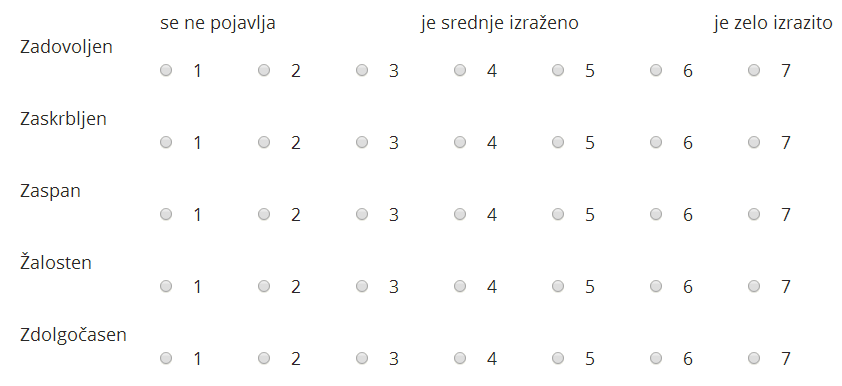
\includegraphics[width=13cm]{images/likart.png}

\caption{Del sedem stopenjske lestvice, s pomočjo katere so udeleženci ocenjevali trenutno razpoloženje. Oznaka 1 pomeni, da se tisto razpoloženje pri udeležencu sploh ne pojavi, 7 pa da je zelo izrazito. }
\label{skala}
\end{figure}

Zanimala nas je tudi struktura vprašalnika, ki je ostala približno enaka v glavnem vprašalniku, s to razliko, da smo tam dodali del z glasbenimi odlomki. Več o tem v poglavju \ref{glavnaanketa}.

Poleg tega smo testirali tudi elemente uporabljene v anketi (sedem stopenjska skala, neskončni barvni krog, izbira z radio gumbi in tekstovnimi polji). Ugotovili smo, da moramo nekatere elemente spremeniti. Spremenili smo barvno skalo, saj smo jo omejili na barvni krog z 49 možnostmi izbire. To je bilo potrebno, ker je imel uporabnik na neskončni skali preveliko možnost izbiranja, obenem pa je bil sistem tri dimenzionalen, kar večina uporabnikov ni opazila in so nastavljali samo odtenek barve, na svetlost in nasičenost pa so pozabili. Skala z 49 možnostmi (prikazana na sliki \ref{colorwheels}) se je izkazala kot boljša alternativa, saj še vedno ponuja veliko možnosti izbire barv, je prijazna uporabniku in pridobljeni podatki so boljši.

Poleg zamenjave barvnega kroga smo zamenjali tudi nekaj ostalih elementov. V delu, kjer uporabnik označi tri svoje najljubše žanre, smo se odločili namesto vpisnih polj ponuditi uporabniku seznam 20 žanrov, iz katerega je izbral in potegnil svoje tri izbire na nov seznam.  Za to smo se odločili, ker so uporabniki v preliminarni analizi v prostor vpisovali tudi žanre, ki niso osnovni in oznake, ki sploh niso žanri. Prav tako nam je preliminarni vprašalnik pomagal izbrati, kateri žanri so tisti, ki jih bomo uporabniku ponudili. Zamenjali smo tudi način, kako uporabnik vnese svoje trenutno razpoloženje in za ta namen uporabili nov element MoodGraph, ki ga bom opisal v poglavju \ref{glavnaanketa}. 

\begin{figure}[ht]
\centering
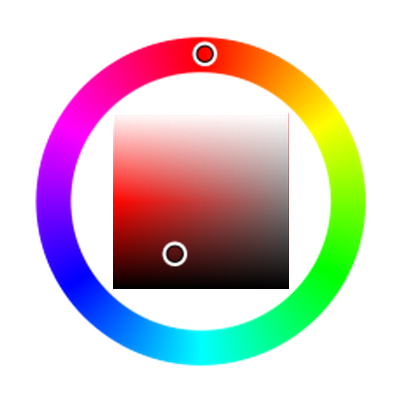
\includegraphics[width=54mm]{colorwheelold.png}
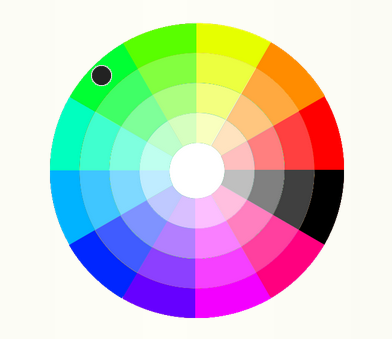
\includegraphics[width=60mm]{colorwheel.png}

\caption{Barvni krog na levi smo uporabili v preliminarni anketi. V zunanjem krogu je bilo možno izbrati odtenek (hue) v notranjem pa je bilo možno izbirati nasičenost in svetlost. Desni krog smo uporabili v glavni anketi. Krog je omogoča izbiro med 49 barvami. Rezina predstavlja en barvni odtenek, proti notranjosti pa se spreminja svetlost in intenzivnost. }
\label{colorwheels}
\end{figure}

\subsection{Glavna anketa}
\label{glavnaanketa}

Glavni vprašalnik, s katerim smo zbrali našo podatkovno zbirko, je bil implementacija preliminarne analize, saj smo v skladu z zbranimi podatki prilagodili oznake in strukturo vprašalnika.

Glavni vprašalnik je bil sestavljen iz treh delov. V prvem delu smo spraševali o uporabnikovih navadah, o poslušanju glasbe in njegovi glasbeni izobrazbi. V drugem delu nas je zanimala predvsem uporabnikova percepcija razpoloženja, glasbe in barv. V tretjem delu so morali uporabniki označiti razpoloženje in barve v odlomku glasbe. 

\textbf{Prvi del} ankete je bil namenjen zajemanja podatkov o  udeleženčevi starosti, spolu in o tem, ali živi na podeželju, ali v mestu.  Uporabnika smo vprašali tudi, če je pod vplivom drog ali drugih substanc. Zanimali so nas podatki o glasbeni izobrazbi in o tem, če udeleženec igra inštrument ali poje, kljub temu da ne obiskuje več glasbene šole ali pa je ni nikoli obiskoval. Poleg tega nas je zanimalo še, koliko časa dnevno uporabnik posluša glasbo in kateri so njegovi najljubši žanri. Izbrati je moral tri svoje najljubše žanre in jih razporediti po priljubljenosti. To smo zajemali s pomočjo elementa prikazanega na sliki \ref{genresel}, kjer je uporabnik izmed nabora 20 žanrov izbral najljubše in jih povlekel v stolpec desno ter razporedil glede na priljubljenost. 

\begin{figure}[h!t]
\centering
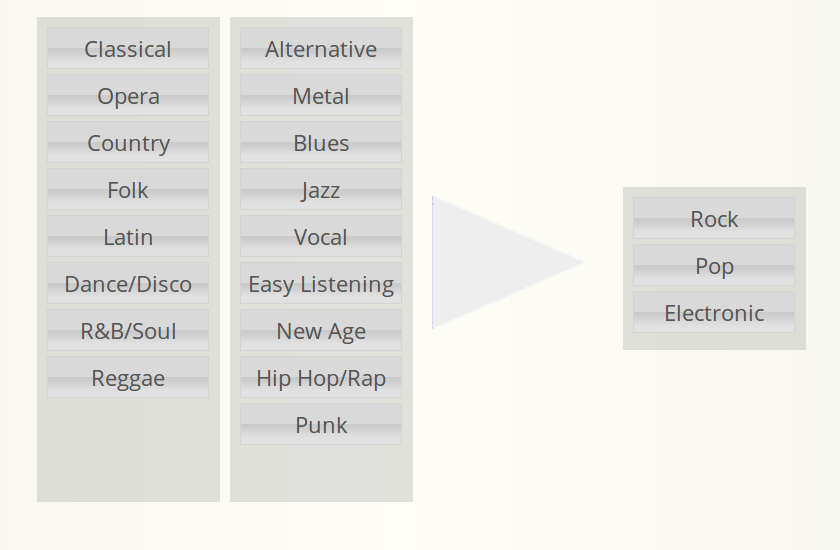
\includegraphics[width=10cm]{genresel.png}

\caption{Element v anketi uporabljen za izbiro najljubših žanrov. Anketiranec je iz levih dveh stolpcev v desnega potegnil do tri izbrane žanre in jih razvrstil po priljubljenosti.}
\label{genresel}
\end{figure}

\textbf{Drugi del} je namenjen ocenjevanju udeleženčevega trenutnega razpoloženja, njegove percepcije oznak za razpoloženje in barve za razpoloženje. Te podatke zajemamo zato, ker nam omogočajo, da ugotovimo povezave med različnimi ocenami razpoloženja v tretjem delu, ki vključuje glasbene odlomke.

Na začetku smo udeleženca vprašali, kako bi svoje razpoloženje označil s točko v prostoru, ki ga označujeta prijetnost in aktivnost (valence-arousal space) \cite{Colibazzi2010}. To je dvodimenzionalen prostor, kjer na vodoravni osi od leve proti desni narašča prijetnost in od spodaj navzgor aktivnost. Svoje razpoloženje je moral udeleženec opisati tudi z izbiro barve s pomočjo barvnega kroga predstavljenega v poglavju \ref{preiliminarnaana}. 

Udeleženec je moral svoje razpoloženje opisati tudi s tem, da je označil, kako je posamezno razpoloženje pri njem izraženo v trenutku reševanja ankete. To smo zajemali s pomočjo novega elementa imenovanega MoodStripe. Potrebno je bilo potegniti posamezne oznake razpoloženj v prostor, kjer od leve proti desni narašča prisotnost posameznega razpoloženja. Če je udeleženec postavil razpoloženje skrajno levo to pomeni, da to razpoloženje pri njem ni prisotno, če pa ga je postavil skrajno desno to pomeni, da je razpoloženje zelo prisotno.

\begin{figure}[ht]
\centering
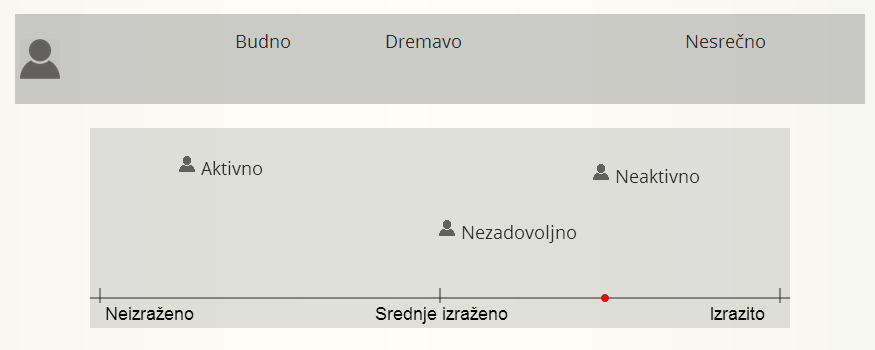
\includegraphics[width=10cm]{images/moodstripe.png}

\caption{Element za zajemanje pristnosti posameznega razpoloženja imenovan moodstripe. Udeleženec je iz zgornjega pravokotnika povlekel razpoloženja in jih vstavil na ustrezno mesto na traku glede na prisotnost posameznega razpoloženja. Prisotnost narašča iz leve (razpoloženje ni izrazito) proti desni (razpoloženje je zelo izrazito). }
\label{moodstripe}
\end{figure}

V drugem delu smo uporabnike povprašali tudi o njihovi percepciji posameznega razpoloženja. Udeleženec je za vsako razpoloženjsko oznako v elementu MoodGraph (slika \ref{moodgraph}) označil, kako prijetno in aktivno je posamezno razpoloženje. Uporabnik je oznake razpoloženj prikazane nad grafom potegnil v to ravnino na, mesto za katerega je mislil, da najbolje opisuje razpoloženje. 

\begin{figure}[ht]
\centering
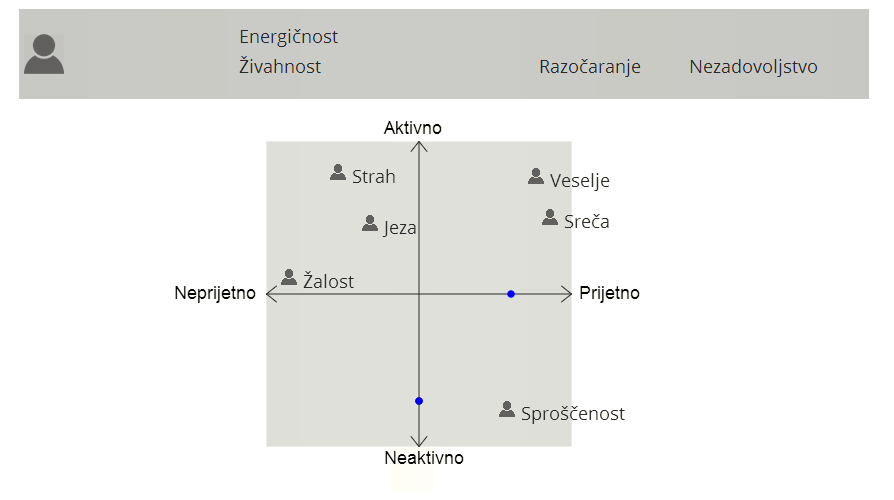
\includegraphics[width=10cm]{images/enomoodgraph.png}

\caption{Enonivojski MoodGraph, element za zajemanje precepcije razpoloženja v VA prostoru. Udeleženec je razpoloženjske oznake uvrstil v graf glede na prijetnost in aktivnost. Prijetnost narašča iz leve proti desni. Aktivnost narašča od spodaj navzgor. }
\label{moodgraph}
\end{figure}

Poleg tega, kako si uporabnik predstavlja posamezno razpoloženje v VA prostoru, nas je zanimalo tudi, kako bi uporabnik opisal ista razpoloženja z barvo. To smo izvedli s pomočjo barvnega kroga (slika \ref{colorwheels}), ki sem ga že opisal zgoraj. 

V \textbf{tretjem delu} smo želeli, da udeleženci za 10 glasbenih odlomkov dolgih 15 sekund označijo razpoloženje, ki ga zaznavajo pri glasbi (percived) in tistega, ki občutijo (induced) ter razpoloženje opišejo z barvo. Odlomki so bili naključno izbrani iz nabora 200 odlomkov. Ker smo se želeli izogniti pristranskosti uporabnika zaradi poznavanja določene glasbe ali dogodkov, ki so se mu zgodili ob poslušanju določene pesmi, smo odlomke izbrali iz zbirk, ki vsebujejo uporabnikom nepoznano glasbo (Jamendo, zbirka s filmsko glasbo, zbirka slovenskih ljudskih pesmi in zbirka moderne elektro-akustične glasbe).  

Glasba je bila izbrana iz štirih različnih virov. Iz odprte podatkovne zbirke Jamendo smo izbrali 80 pesmi, ki so bile iz različnih žanrov in dokaj vsakdanje. Naslednjih 80 pesmi smo vzeli iz zbirke filmske glasbe opisane v \cite{Eerola2010}. Dodali smo še 20 slovenskih ljudskih pesmi in 20 pesmi iz nabora moderne elektro-akustične glasbe. Uporabnikov nismo želeli preveč obremeniti, zato je bilo vsakemu uporabniku naključno dodeljenih zgolj 10 odlomkov.

Pri vsakem odlomku je udeleženec označil, katera razpoloženja so izražena v odlomku, katera razpoloženja posamezna glasba vzbudi v njem in s katero barvo iz barvnega kroga (slika \ref{colorwheels}) bi posamezno pesem opisal. Razpoloženja izražena v odlomku je izbiral iz nabora 14 oznak, razpoloženja, ki jih je glasba pri njem vzbudila, pa iz nabora 10 oznak. Udeleženec je lahko za posamezen odlomek izbral več oznak iz obeh naborov. Poleg tega, da je izbral posamezno oznako jo je moral še uvrstiti v VA prostor. S tem smo zajeli tudi podatek kako si predstavlja določeno oznako pri posamezni pesmi. Na primer, pri neki pesmi je lahko veselje zelo aktivno, pri drugi pa manj. Poleg tega nam ta podatek omogoča, da raziskujemo tudi, kako si uporabnik v VA prostoru predstavlja posamezno pesem. Za zajemanje tega podatka smo uporabili dvokategorni MoodGraph prikazan na sliki \ref{moodgraphdvo}.

\begin{figure}[htb]
\centering
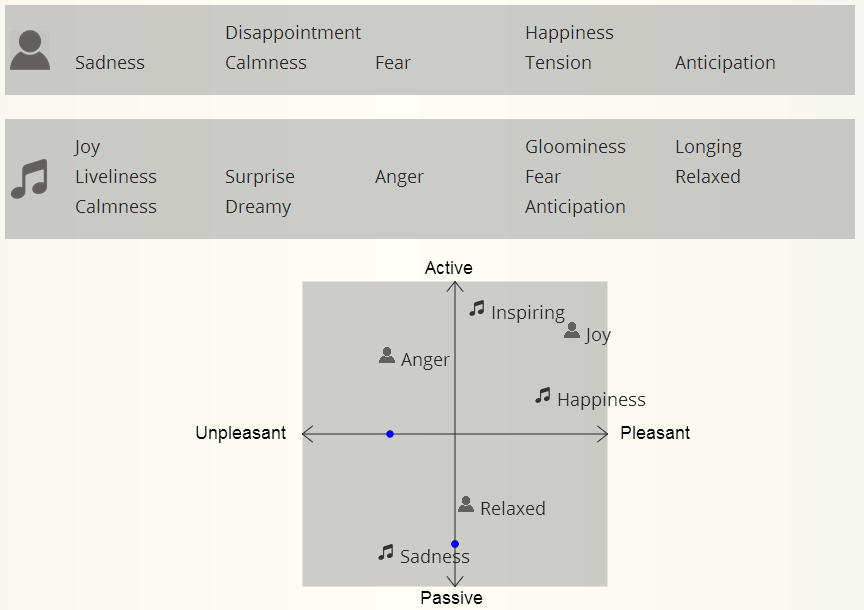
\includegraphics[width=10cm]{images/moodgraphdvo.png}

\caption{Dvonivojski MoodGraph, element za zajemanje razpoloženja v glasbi in njegovo umestitev v VA prostor. Nota označuje nabor razpoloženj, ki jih udeleženec zazna v glasbi (percived). Figura človeka označuje nabor razpoloženj, ki jih udeleženec občuti (induced). Udeleženec je iz vsake skupine razpoloženj izbral tista, ki po njegovem izražene ali vzbujene in jih umestil na v VA prostor glede na prijetnost in aktivnost.}
\label{moodgraphdvo}
\end{figure}

\section{Implementacija ankete}

Anketo smo implementirali v obliki spletne aplikacije. Za osnovo spletne aplikacije smo izbrali okolje CodeIgniter. Gre za odprto kodno okolje, ki je namenjeno za izdelavo spletnih aplikacij. Narejen je na osnovi PHP jezika in uporablja princip MVC (model-view-controller). Princip MVC pomeni, da je aplikacija razdeljena v tri dele. Model skrbi za povezavo s podatkovno bazo, view skrbi za prikaz podatkov uporabniku, med tem ko controller upravlja s podatki in skrbi za delovanje aplikacije.

Za implementacijo same ankete smo uporabili tehnologije HTML5, javascript, jQuery in xml zapis. Anketa je sestavljena tako, da se dinamično generira na podlagi podatkov iz xml dokumenta. Na tak način smo naredili okolje, kjer za kreiranje nove ali popravljanje obstoječe ankete ni potrebno ročno sestavljati html dokumenta. Zaradi takega načina implementacije bo sistem možno uporabiti še za druge ankete, saj je zelo splošen. Elementi ankete se dinamično generirajo s pomočjo javascript skripte, ki uporablja tudi elemente jQuerya. Anketa poleg klasičnih tekstovnih polj, radio gumbov in izbirnih seznamov vsebuje tudi elemente, ki smo jih načrtovali sami. Element za izbiro najljubšega žanra, MoodGraph in MoodStripe predstavljeni v poglavju \ref{glavnaanketa} so načrtovani z uporabo HTML5 canvasa in jQuery Draggable funkcionalnosti. Prav tako je na podlagi HTML5 canvasa in jQuery poslušalcev za klik načrtovan element za izbiro barv. 

Za preverjanje pravilnosti vnosa smo uporabljali HTML5 funkcionalnost za klasične elemente (vnosno polje, izbirni seznam in radio gumbi) in preverjanje z uporabo javascript skripte za elemente, ki smo jih načrtovali sami (MoodGraph, MoodStripe, element za izbiro žanra in element za izbiro barve). Rezultate smo shranjevali v MySQL podatkovno bazo z uporabo funkcij, ki jih prinaša model v CodeIgniterju. 


\section{Sestava podatkovne zbirke}

Struktura podatkovne zbirke sledi strukturi uporabljene ankete, zato je razdeljena v tri dele.  V prvem delu smo zbrali 1423 odgovorov in s tem tudi toliko vpisov v našo zbirko. V drugem delu je vpisov 1090. V tretjem delu, kjer je moral udeleženec oceniti 10 pesmi, smo zbrali 7187 odgovorov. Ta del je izpolnjevalo 741 udeležencev.

V prvem delo so podatki, ki opisujejo udeležence (podrobnosti so predstavljene v tabeli \ref{prvidel}). Za vsakega udeleženca zbirka vsebuje podatek o starosti na leto natančno, o spolu in o tem ali živi na podeželju ali v mestu. Poleg tega smo zbrali podatke o tem, koliko časa se ukvarja z glasbo, koliko časa je hodil v glasbeno šolo do leta natančno ter koliko časa na dan posluša glasbo. Tukaj je uporabnik poslušanje glasbe uvrstil v eno od kategorij: do 1 ure, od 1 do 2 uri, od 2 do 3 ure in več kot 3 ure. Imamo tudi podatek o najljubših glasbenih žanrih udeleženca. Udeleženec je podal najmanj en in največ tri žanre. Zanimalo nas je še psihofizično stanje udeleženca med reševanjem. Torej imamo podatek ali jemlje zdravila, ki vplivajo na razpoloženje ter, če je bil v trenutku reševanja pod vplivom drog ali alkohola. 

Drugi del podatkovne zbirke vsebuje podatke o udeleženčevem razpoloženju v trenutku, ko je izpolnjeval anketo in o tem kako si udeleženec predstavlja posamezna razpoloženja. Uporabnikovo razpoloženje opisujejo trije podatki. Prvi je točka v VA prostoru (x in y koordinata). Drugi je barva v barvnem krogu (tukaj hranimo podatek o tem, katero barvo je  udeleženec izbral). Tretji pa je vrednost, kako močno je posamezno razpoloženje iz nabora 17 razpoloženj, izraženo pri udeležencu v tistem trenutku. Hranimo vrednost med 0 in 1 za vsako razpoloženje. Kot smo že omenili, drugi del vsebuje tudi podatek o tem, kako si udeleženec predstavlja razpoloženja. Za nabor 10 razpoloženj imamo podatek, kam v VA prostoru spada to razpoloženje po mnenju udeleženca in barvo, s katero ga je udeleženec označil. 

Tretji del podatkovne zbirke je malo drugačen. Tu nimamo le enega odgovora na od posameznega udeleženca, ampak do 10 odgovorov, za vsako pesem en odgovor. Imamo podatek o tem, katera razpoloženja so izražena v glasbi in katera razpoloženja glasba vzbudi pri udeležencu. Izbrana razpoloženja je udeleženec umestil v VA prostor, zato imamo tudi podatek, kam v tem prostoru se umeščajo.  Za vsako pesem imamo tudi podatek o barvi, s katero je udeleženec označil glasbeni odlomek.  



\begin{table}[H]
\begin{center}
\caption{Vprašanja prvega dela ankete. Tabela poleg vprašanj vsebuje še podatke o možnih odgovorih in komentar. V prvem delu ankete smo pridobivali demografske podatke in podatke o uporabnikovih izkušnjah z glasbo.}
\begin{tabular}{| p{3.5cm} | p{4.5cm} | p{4.5cm} |}
\hline
Vprašanje & Odgovori & Komentar \\ \hline \hline
Starost & [5, 99] & izražena v letih \\ \hline
Spol & \{Moški, Ženski\} & \\ \hline
Področje prebivanja & \{mesto, podeželje\} & \\ \hline
Leta glasbenega izobraževanja & [0, 20] & v letih, 0 - pomeni, da se ni glasbeno izobraževal \\ \hline
Igranje inštrumenta ali petje & [0, 20] & v letih, 0 - pomeni, da se nikoli ni ukvarjal z glasbo \\ \hline
Uživanje drog & \{da, ne\} & \\ \hline
Vpliv drog & \{da, ne\} &  Je bil udeleženec pod vplivom drog med reševanjem ankete? \\ \hline
Najljubši žanri & \{classical, opera, country, folk, latin, dance/disco, electronic, RnB/soul, hip hop/rap, reggae, pop, rock, alternative, metal, blues, jazz, vocal, easy listening, new age, punk\} & Udeleženec je moral izbrati do tri žanre (najmanj enega) in jih razvrstiti od najljubšega do najmanj priljubljenega. \\ \hline
Čas poslušanja glasbe & \{manj kot 1, 1-2, 2-3, več kot 3\} & v urah na dan \\ \hline

\end{tabular}
\label{prvidel}
\end{center}
\end{table} 

\begin{table}[H]
\begin{center}
\caption{Vprašanja drugega dela ankete. Tabela vsebuje vprašanja, možne odgovore in komentar. Vprašanja sprašujejo po udeleženčevem razpoloženju, percepciji razpoloženja in povezavi med barvami in razpoloženjem.}
\begin{tabular}{| p{3.5cm} | p{4.5cm} | p{4.5cm} |}
\hline
Vprašanje & Odgovori & Komentar \\ \hline \hline
Trenutno razpoloženje v VA prostoru & VA prostor & Uporabnik je označil razpoloženje v VA prostoru, predstavljenem v poglavju \ref{glavnaanketa}. \\ \hline
Barva razpoloženja & Barvni krog & Uporabnik je izbral barvo trenutnega razpoloženja z barvnim krogom predstavljeni v poglavju \ref{preiliminarnaana}. \\ \hline
Percepcija razpoloženja & \{strah, energičnost, jeza, sproščenost, sreča, žalost, živahnost, veselje, razočaranje, nezadovoljstvo\} & Uporabniki so umestili razpoloženja v VA prostor z uporabo MoodGrapha predstavljenega v poglavju \ref{glavnaanketa} \\ \hline
Trenutno razpoloženje z oznakami & \{aktivno, budno, dremavo, neaktivno, nesrečno, nezadovoljno, razočarano, sproščeno, srečno, utrujeno, vedro, veselo, zadovoljno, žalostno, mirno, jezno\} & Uporabnik je razvrstil vse oznake na MoodStripe (predstavljen v poglavju \ref{glavnaanketa}), glede na prisotnost od neizraženega do zelo izraženega. \\ \hline
Barva razpoloženja & \{sreča, žalost, nezadovoljstvo, energičnost, razočaranje, veselje, sproščenost, živahnost, strah, jeza\} & Za vsako razpoloženje je uporabnik izbral barvo, ki ga najbolj opisuje z uporabo barvnega kroga. \\ \hline

\end{tabular}
\label{drugidel}
\end{center}
\end{table}

\section{Analiza podatkov}

\subsection{Demografska analiza}

Povprečna starost udeležencev je 26,5 let. Najmanjši udeleženec je bil star 15 let, najstarejši pa 64 let. Največ udeležencev je bilo starih 20 let. Anketo je rešilo več udeleženk ženskega spola, kar 65\%. Večina udeležencev prihaja iz urbanega okolja, 66\% udeležencev živi v mestu in 34\% na podeželju.

\paragraph{Ukvarjanje z glasbo}

Zanimivo je, da ima kar polovica vseh udeležencev glasbeno izobrazbo, z glasbo pa se ukvarja 53\% udeležencev (igrajo inštrument ali pojejo). Udeleženci, ki so obiskovali glasbeno šolo, so jo v povprečju obiskovali 6 let. Tisti, ki se z glasbo ukvarjajo neformalno se z njo ukvarjajo povprečno 11 let. Pričakovano igranje inštrumenta in petje ter leta glasbene šole zelo visoko korelirata (r=0,653). Iz slike \ref{ukvarjanjeglizobrazba} poleg korelacije razberemo tudi, da se večina ljudi z glasbo ukvarja tudi po dokončani formalni izobrazbi, kar sklepamo iz podatka, da se večina ljudi z glasbo ukvarja dlje, kot traja zgolj formalna izobrazba. 

\begin{figure}[hbt]
\centering
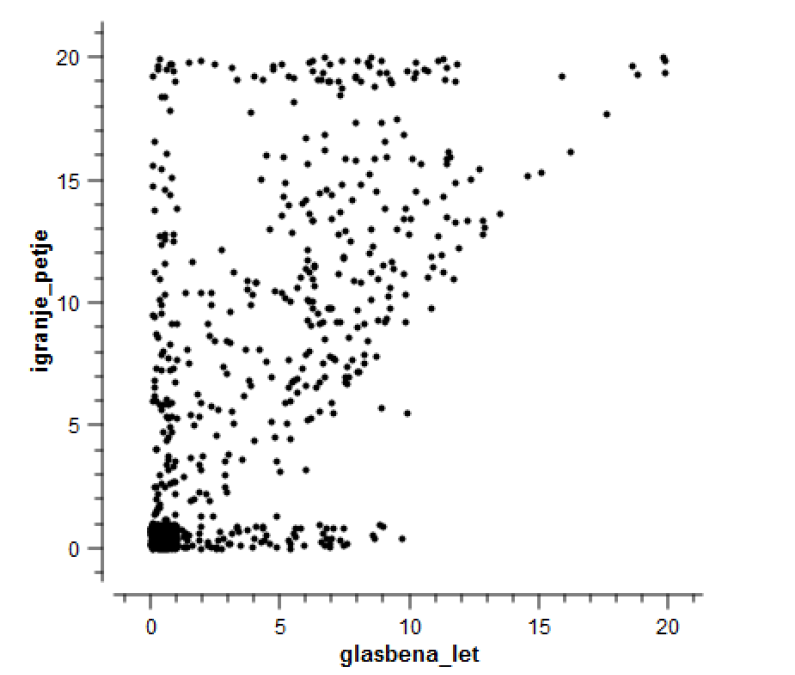
\includegraphics[width=10cm]{images/izobrazba_ukvarjanje.png}

\caption{Vsaka točka na sliki prikazuje povezavo med trajanjem formalnega glasbenega izobraževanja na vodoravni osi in leta ukvarjanja z glasbo (igranje inštrumenta ali petje) na navpični osi.  Iz slike je razvidno, da se večina udeležencev tudi po končani formalni izobrazbi ukvarja z glasbo.  }
\label{ukvarjanjeglizobrazba}
\end{figure}

Največ udeležencev posluša glasbo 1 do 2 uri na dan, najmanj pa 2 do 3 ure na dan. Količina poslušanja glasbe ne korelira z nobeno od ostalih demografskih spremenljivk. 

\paragraph{Zdravila in droge}

Zdravila, ki vplivajo na razpoloženje, uživa 4,2\% udeležencev. Kar 3\% udeležencev je poročalo, da so bili med reševanjem ankete pod vplivom drog ali alkohola. Tudi ta dva parametra visoko korelirata med seboj (r = 0,519).

\paragraph{Žanri}

Kot je razvidno iz grafa na sliki \ref{zanrigraf}, je večina udeležencev kot najljubši žanr označila rock (31,6\% udeležencev). Na drugem mestu med najljubšimi žanri je pop z 16,6\% in na tretjem alternativna glasba. Na zadnjih dveh mestih sta opera in reggae, ki sta najljubši žanr manj kot odstotku vprašanih. Razporeditev žanrov, ki so jih uporabniki uvrstili na prvo mesto, ni enakomerna, saj kot največkrat izbrana žanra zelo izstopata rock in pop.  

Na drugo mesto je spet največ vprašanih uvrstilo rock (20\% vprašanih), drugi največkrat uvrščen žanr na drugo mesto je pop z 13,9\%. Najmanjkrat izbran žanr je opera. Na drugem mestu so izbire že bolj raznolike kot pri najljubšem žanru, vendar vrh še vedno izstopa. 

Zanimivo je, da je največ udeležencev na tretje mesto uvrstilo klasično glasbo. Za to izbiro se je odločilo 11,9\% udeležencev. Klasiki sledi rock (11,3\%). Najredkeje so udeleženci na tretje mesto uvrstili new age in punk. Za izbire na tretjem mestu je značilno, da so bolj raznolike, saj noben žanr ne izstopa. 

\begin{figure}[hbt]
\centering
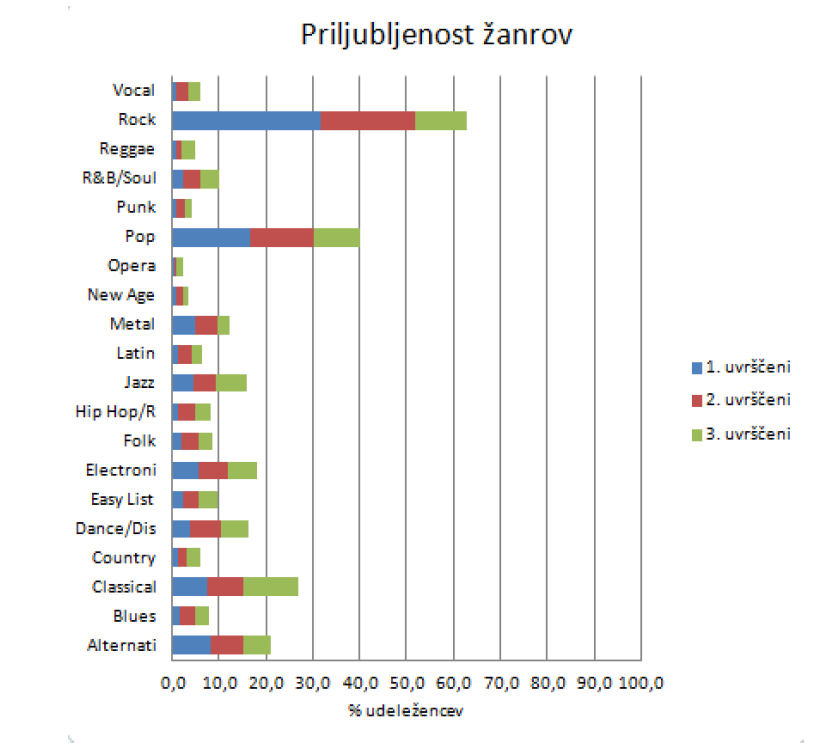
\includegraphics{images/genre.png}

\caption{Priljubljenost žanrov ter uvrstitev teh na prvo, drugo ali tretje mesto. Razvidno je, da je najbolj priljubljen žanr rock, sledi mu pop in klasična glasba. Najmanj popularen žanr je opera.}
\label{zanrigraf}
\end{figure}

Izmed vseh žanrov smo potem izbrali najbolj priljubljene: rock, pop, country, alternativna glasba in klasična glasba. Naredili smo primerjavo med najljubšimi žanri po starostnih skupinah (slika \ref{zanrigraftop}). Udeležence smo razdelili v 6 starostnih skupin. Vsaka od skupin zajema 10 let. Pri vseh starostnih skupinah je popularna rock glasba. Pri najmlajših štirih starostnih skupinah je na prvem mestu. Tudi pop glasba se pojavi pri vseh skupinah razen najstarejših dveh. Razlike se pojavijo v ostalih žanrih. Pri mlajših so popularni še žanri kot so metal, alternative in elektronska glasba. Pri starejših je zelo popularna klasična glasba. V najstarejših dveh skupinah se pojavi na prvem mestu. V teh skupinah so popularne še folk, jazz in country. Srednji dve starostni skupini pa sta kombinacija obojega. V njih se pojavi še alternativna glasba in tudi jazz ter klasična glasba. 

\begin{figure}[hbt]
\centering
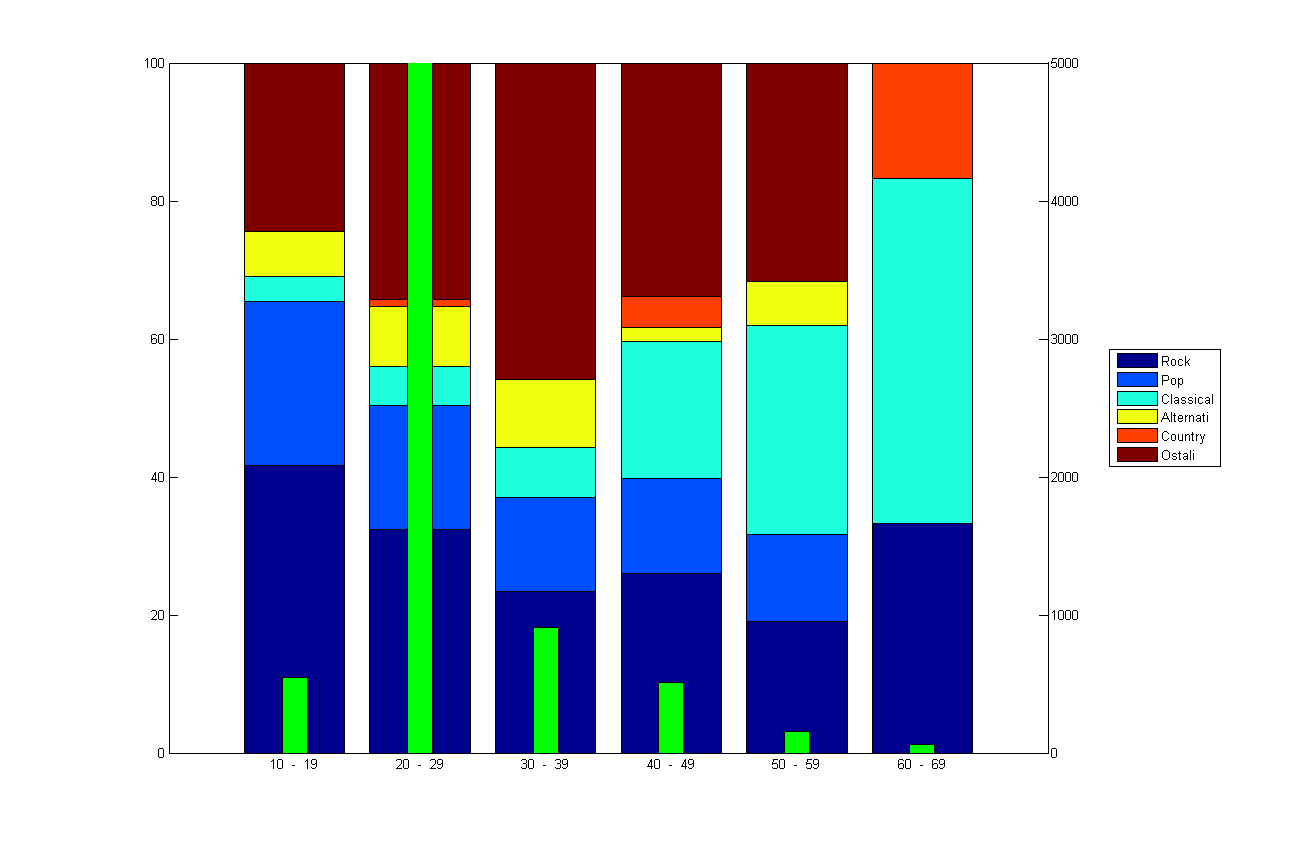
\includegraphics[width=15cm]{images/genretop1.png}

\caption{Priljubljenost posameznih glasbenih žanrov po starostnih skupinah. Na vodoravni osi so označene starostne skupine. Širši stolpci predstavljajo razporeditev posameznih žanrov v odstotkih, zeleni pa število udeležencev v posamezni starostni skupini.  }
\label{zanrigraftop}
\end{figure}

Naredili smo tudi analizo priljubljenosti glede na spol. Ugotovili smo, da je pri obeh spolih enako zastopana rock glasba. S tem, da pri udeležencih prevladuje še elektronska glasba in metal. Pri udeleženkah pa je na prvem mestu pop glasba. 


\subsection{Razpoloženje, čustva in barva}
\label{razcusbar}

Za ta del analize smo iz podatkovne zbirke odstranili vse, ki so bili pod vplivom drog ali zdravil, ki vplivajo na razpoloženje. V anketi smo udeleženčevo trenutno razpoloženje zajemali na dva načina. Najprej je udeleženec moral označiti svoje razpoloženje v VA prostoru. Torej je označeval prijetnost in aktivnost trenutnega razpoloženja. Sledila so tudi vprašanja, kjer je udeleženec trenutno razpoloženje ocenjeval z tem, da je označil, v kakšni meri je prisotno posamezno razpoloženje pri njem. Zanimala nas je predvsem korelacija med prisotnostjo posameznih razpoloženj in med koordinatama v VA prostoru. Kot je razvidno iz slike \ref{prisotnost_kor} je prijetnost (koordinata x) najmanj oddaljena od razpoloženj: sproščenost, sreča, zadovoljstvo, vedrost in veselje. Vrednosti predstavljene s y-koordinato se po pričakovanjih najbolje podobne z razpoloženjem aktivnost. Prijetnost (predstavljena s x-koordinato) se najmanj ujema s razpoloženji nesrečno, nezadovoljno in razočarano, kar je bilo pričakovati, saj je prijetnost (x-koordinata) ravno nasprotna s tem razpoloženjem. S koordinato y se pričakovano najmanj ujema razpoložene neaktivno zaradi enakega razloga kot pri koordinati x.Opazimo lahko tudi dobro ujemanje med razpoloženji nezadovoljno in razočarano ter med razpoloženji veselo in zadovoljno. 

\begin{figure}[hbt]
\centering
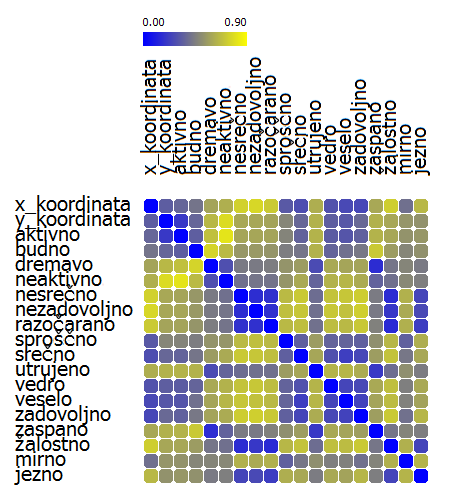
\includegraphics[width=10cm]{images/korelacija.png}

\caption{Povprečna evklidska razdalja med posamezni atributi. Iz slike je razvidno, da je prijetnost najbolj podobna z razpoloženji: sproščenost, sreča, zadovoljstvo, vedrost in veselje. Aktivnost (koordinata y) se najbolje ujema z razpoloženji aktivno, vedro, veselo in zadovoljno. Opazimo lahko tudi ujemanje med razpoloženji nezadovoljno in razočarano ter veselo in zadovoljno.}
\label{prisotnost_kor}
\end{figure}

Slika \ref{razpolozenjeva} prikazuje kako so ljudje umestili svoje razpoloženje v VA prostor. Opazno je, da so se udeleženci v večjem številu umestili v desno polovico koordinatnega sistema, kar pomeni, da so svoje razpoloženje označili kot bolj prijetno. Več udeležencev občuti bolj neaktivno razpoloženje, kar se odraža v tem, da je več udeležencev svoje razpoloženje uvrstilo v spodnji del koordinatnega sistema. Največja gostota razpoloženj udeležencev se nahaja v spodnjem desnem kvadrantu, kar pomeni, da se počutijo bolj prijetno in so bolj neaktivni. 

Zelo zanimivo je, da s koordinato y korelira starost in tudi poslušanje glasbe. Tisti, ki so starejši, so označili, da se počutijo manj aktivne in obenem manj poslušajo glasbo. 

\begin{figure}[hbt]
\centering
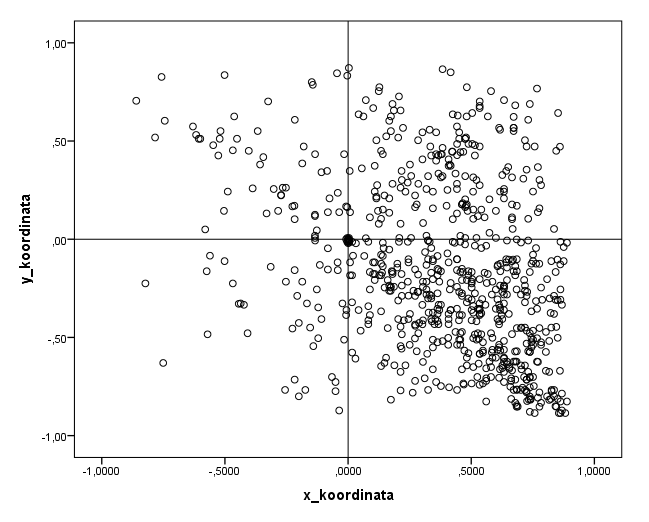
\includegraphics[width=10cm]{images/vamood.png}

\caption{Slika prikazuje odgovore vseh uporabnikov o razpoloženju v VA prostoru. Vidi se, da je bilo največ udeležencev v času reševanja ankete prijetnega in neaktivnega razpoloženja.  }
\label{razpolozenjeva}
\end{figure}

V anketi smo spraševali tudi o tem, kako uporabniki dojemajo posamezno razpoloženje. Razpoloženje so morali opisati tako, da so posamezno oznako postavili v VA prostor. Na sliki \ref{moodperception} je prikazana umestitev 8 razpoloženj v VA prostor. 

Slika levo zgoraj prikazuje primerjavo med razpoloženjema strah in sreča. Strah je zelo neprijetno razpoloženje, sreča pa prijetno. Oba sta razporejena praktično preko celotne y osi, kar si lahko razlagamo s tem, da sta to razpoloženji, za katera je težko določiti ali sta aktivni ali ne. 

Iz slike desno zgoraj je po pričakovanjih razvidno, da je energičnost zelo prijetno in aktivno razpoloženje, obenem pa je žalost neprijetna in neaktivna. Zanimivo je, da je kar nekaj uporabnikov označilo, da je žalost aktivno razpoloženje.

\begin{figure}[!hbt]
\centering
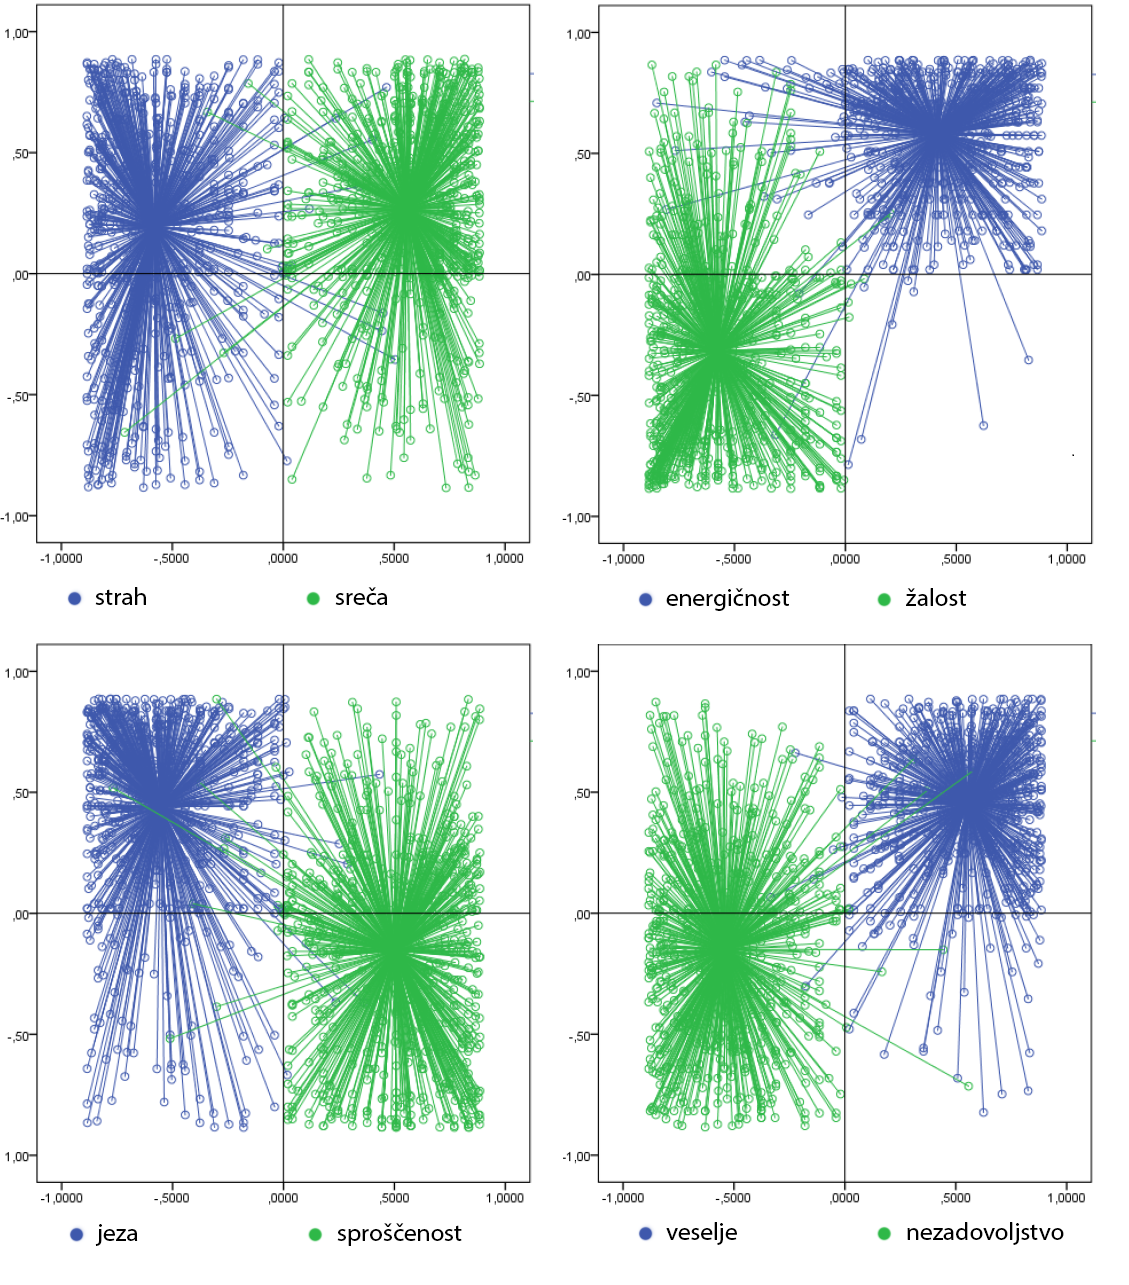
\includegraphics[width=12cm]{images/vamoodlables.png}

\caption{V zgornjih VA prostorih je prikazana razporeditev 8 razpoloženj, glede na to, kako so jih v ta prostor uvrstili udeleženci. V splošnem je opazno, da so se udeleženci glede prijetnosti odločili dokaj enotno, medtem ko so večje razlike v aktivnosti.}
\label{moodperception}
\end{figure} 

Na tretjem grafu (levo spodaj) je narejena primerjava med jezo in sproščenostjo. Jeza je po pričakovanjih zelo aktivno in negativno razpoloženje, čeprav je zanimivo, da nekaj udeležencev meni, da je neaktivna. Sproščenost je prijetna in glede na aktivnost razporejena preko celotnega prostora, čeprav prevladuje mnenje, da je bolj neaktivno razpoloženje. Tukaj je tudi veliko odgovorov, ki so nevtralni.

Iz četrte slike je razvidno, da je veselje zelo prijetno in aktivno razpoloženje, medtem ko je nezadovoljstvo neprijetno. Po aktivnosti je nezadovoljstvo bolj razpršeno, kar govori o tem, da je ta parameter pri tem razpoloženju težje določiti.

\begin{figure}[!hbt]
\centering
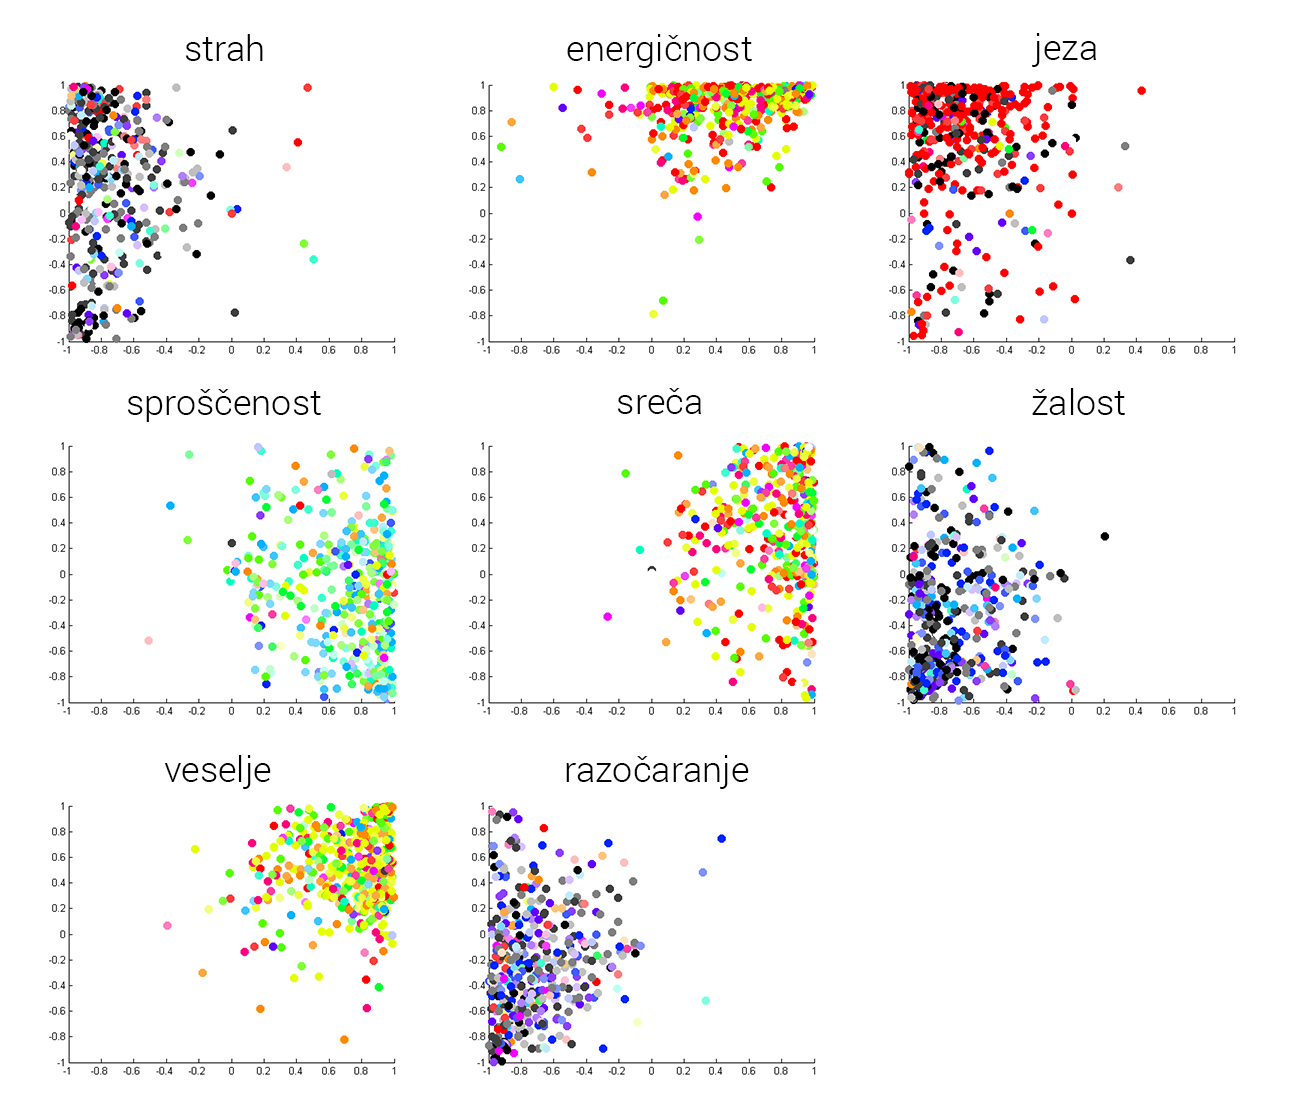
\includegraphics[width=14cm]{images/mood_color.png}

\caption{Izbira barv za posamezna razpoloženja in umestitev razpoloženj v VA prostor. Iz slike je razvidno, da so pri prijetnih razpoloženjih izbrane barve manj intenzivne, odtenki so v tem primeru večinoma rdeči, rumeni in zeleni. Pri neprijetnih razpoloženjih so izbrani bolj intenzivni in temnejši odtenki.}
\label{moodcolor}
\end{figure} 

\paragraph{Barva}

Ugotovili smo, da obstaja zelo dobra korelacija med barvo in  pozicijo razpoloženja v VA prostoru, kar je možno opaziti na sliki \ref{moodcolor}. Pri prijetnih razpoloženjih se barva v večini primerih giblje med rdečo in nežno modro. Pri neprijetnih razpoloženjih so odtenki večinoma modri, črni, rdeči in vijolični. Barve so tu zelo intenzivne.

Iz slike \ref{moodcolor} je razvidno da so bili pri strahu pogosto izbrani bolj sivi in črni odtenki. Veselje je bilo v večini primerov označeno z bolj intenzivnimi toni. Odtenki so bili v tem primeru rdeči, oranžni, rumeni ter svetlo zeleni. Pri energičnosti se je večina uporabnikov odločila za rdečo, zeleno in rumeno barvo. Za sproščenost je zanimivo, da je dokaj enakomerno razporejena preko celotnega barvnega spektra. Torej si to razpoloženje vsak udeleženec predstavlja drugače. Intenzivnost barv je pri sproščenosti manjša. Pri jezi je bila pogosto izbrana rdeča, modra ali vijolična barva. Izbirali so praktično med vsemi intenzivnostmi.


\subsection{Glasba, razpoloženje in barva}

\begin{figure}[hbt]
\centering
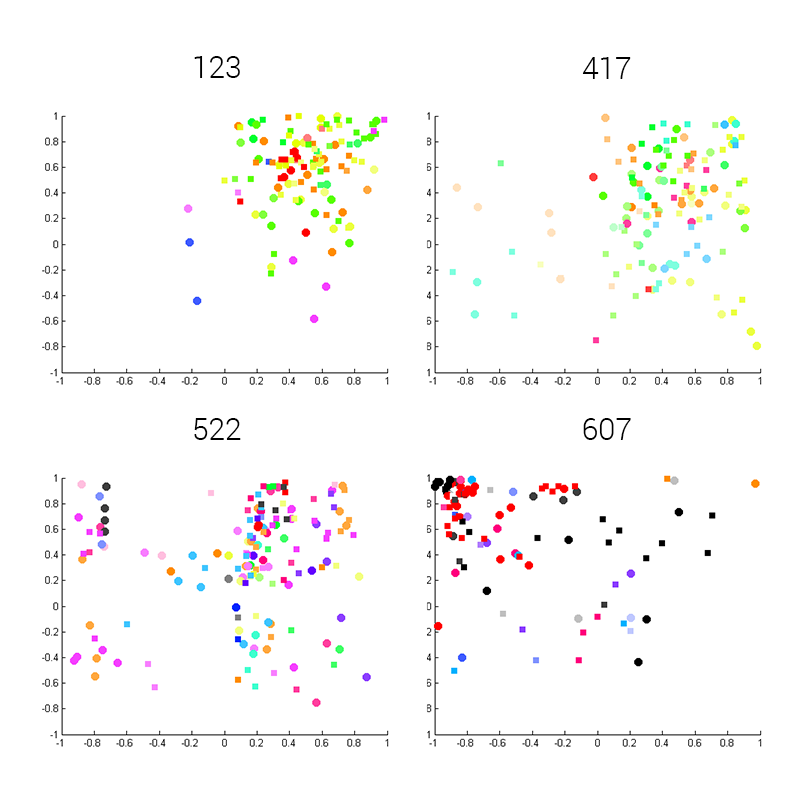
\includegraphics[width=12.5cm]{images/moodmusic.png}

\caption{Prikaz razpoloženj v VA prostoru skupaj z barvami, s katerimi so razpoloženja označili uporabniki. S krogi so označena razpoloženja, ki jih po njihovem mnenju glasba vzbudi pri poslušalcu, z kvadrati pa razpoloženja, ki so izražena v glasbi. Narejen je prikaz za 4 pesmi. Nad slikami so označene identifikacijske številke pesmi. Prva pesem je iz zbirke filmske glasbe (identifikacijska številka se začne z 1), druga je iz zbirke etnografskih pesmi (identifikacijska številka se začne z 4), tretja iz zbirke Jamendo (identifikacijska številka se začne z 5) in četrta iz nabora moderne računalniške glasbe (identifikacijska številka se začne z 6).}
\label{moodmusic}
\end{figure} 

Za konec smo izbrali še 4 glasbene odlomke in v sliki \ref{moodmusic} prikazal rezultate. Predstavili smo VA vrednosti, kamor so udeleženci postavili razpoloženja, ki nastopajo v posamezni pesmi. Z krogci so označena mesta kamor so postavili razpoloženja, ki jih po njihovem mnenju glasba vzbudi pri človeku. Z kvadratki so predstavljena razpoloženja, ki jih pesem izraža. Obenem smo vizualizirali tudi barve, ki po mnenju uporabnikov opisujejo posamezno pesem. 

Pri prvi pesmi nastopajo razpoloženja, ki so bolj pozitivna in aktivna (večina oznak se nahaja desno zgoraj). Tudi barve so glede na analizo barv zgoraj temu primerne, saj so svetle in niso tako intenzivne, kar se ujema z bolj aktivnimi razpoloženji. Iz grafa se opazi, da ljudje bolj poenoteno dojemajo čustva, ki naj bi jih glasba izražala, manj enotni pa so si v čustvih, ki jih ob poslušanju doživljajo. 

Pri drugi pesmi (desno zgoraj) so razpoloženja še vedno bolj prijetna in tudi malo bolj aktivna kot neaktivna. Tudi barve so enako kot pri prejšnji sliki temu primerne. V primerjavi s prejšnjo pesmijo pa so udeleženci veliko bolj neodločeni glede aktivnosti v pesmi. Tudi pri tej pesmi so izražena razpoloženja manj razpršena in se v večini nahajajo v zgornjem desnem delu grafa za razliko od tistih, ki jih pesem vzbuja. 

Pri pesmi na grafu levo spodaj odločitve niso tako enotne. V večji meri prevladujejo prijetna in obenem aktivna razpoloženja. Je pa zanimivo, da se pojavijo 4 gruče odgovorov. Prva je skrajno levo zgoraj, druga levo spodaj, tretja največja je desno zgoraj in četrta desno spodaj. Zanimivo je, da so odločitve o izraženih razpoloženjih z nekaj izjemami bolj aktivne, tiste o vzbujenih pa se v večji meri pojavijo tudi v ostalih delih prostora. 

Graf za četrto pesem (desno spodaj) pa je pravo nasprotje vsem ostalim. Notri nastopajo zelo neprijetna razpoloženja, ki pa so v večini primerov aktivna. Značilno je, da je večina ljudi prijetnost in tudi aktivnost označila na skrajnem robu prostora. V tem primeru so izražena razpoloženja bolj razpršena kot tista, ki jih glasba vzbudi. Tudi barve pri tem grafu s primerne izbranim razpoloženjem, saj so bolj intenzivne in predvsem v rdeče črnih odtenkih. 

\chapter{Algoritmi za ocenjevanje razpoloženja v glasbi}

Zadali smo si, da preizkusimo delovanje nekaterih algoritmov za ocenjevanje razpoloženj v glasbi. V tem poglavju bomo predstavili delovanje in rezultate za regresijski algoritem in algoritem Gaiatransform iz knjižnice Essentia.

\section{Regresijski algoritem}
\label{regresijsialg}

Prvi algoritem, ki smo ga preizkusil je algoritem, ki so ga implementirali Schmidt et al. \cite{schmidt2009projection}. Ni nam uspelo dobiti izvirnega algoritma avtorja. Po informacijah, ki smo jih pridobil ob natančnem pregledu avtorjevega članka in nekaj izmenjanih e-poštah z avtorjem, smo sami implementiral algoritem, po navodilih avtorja. Algoritem iz glasbe izračuna značilnice. Na podlagi teh pa potem napove prijetnost (valence) in aktivnost (arousal) v skladbi. 

Algoritem za delovanje potrebuje značilnice izračunane na podlagi glasbenih odlomkov. Uporabili smo značilnici MFCC \cite{logan2000mel} in kromatski vektor \cite{Bello2005}. Za računanje teh vrednosti smo uporabili Python knjižnico LibROSA. Poleg tega smo potrebovali še že znane VA vrednosti za del odlomkov, da na podlagi tega učimo algoritem. V našem primeru smo imeli za vse odlomke znane VA vrednosti, tako smo lahko naključno določili, na katerem delu podatkovne zbirke bomo učili algoritem in na katerem delu testirali. Obenem smo na tak način lahko preverili natančnost naših napovedi. VA vrednosti smo izračunali za vsako pesem s povprečenjem vrednosti v podatkovni zbirki opisani v poglavju \ref{odatasetu}.

Algoritem deluje, tako da glasbene odlomke naključno razdeli na dva dela. 70\% podatkovne odlomkov uporabi za učenje in ostalih 30\% za testiranje. Na delu zbirke za učenje potem uporabi metodo najmanjših kvadratov (Least squares method) \cite{abdi2007method}, s katero izračuna vektor $b$, ki ga potem uporabimo za preslikovanje iz matrike z značilnicami v VA vrednosti z enačbo \ref{regresion}. Metoda najmanjših kvadratov kot vhod vzame matriko z značilnicami za posamezno pesem in vektor z VA vrednostmi. Ta postopek izvajamo ločeno za prijetnost (valence) in aktivnost (arousal).  

\begin{equation} 
\label{regresion}
y = X \cdot b
\end{equation} 

V enačbi \ref{regresion} je $X$ matrika, ki v vsaki vrstici vsebuje značilnice za posamezen glasbeni odlomek, $b$ je vektor, ki preslikuje iz prostora, ki ga predstavljajo značilnice v VA vrednost. Vrednost, ki jo algoritem napove je $y$. Vsaka vrednost predstavlja prijetnost ali aktivnost za en glasbeni odlomek. 

\subsection{Rezultati za regresijski algoritem}

Algoritem smo kot sem že omenil učili z 70\% glasbenih odlomkov, test pa smo izvedli na 30\% odlomkov. Te napovedi, ki jih je algoritem dal na testnih odlomkih, smo potem primerjali s podatki za vsako pesem iz podatkovne zbirke.

Rezultati so predstavljeni v tabeli \ref{regressionresults} za oba tipa značilnic (MFCC in kromatski vektor) posebej. Za vsak primer smo izračunali povprečno razdaljo med povprečno vrednostjo iz podatkovne zbirke in algoritmično napovedano vrednostjo. Prav tako smo izračunali povprečno razdaljo med najbližjo točko v podatkovni zbirki in napovedano vrednostjo. Povprečno razdaljo do povprečne vrednosti smo izrazili tudi v večkratniku standardnega odklona v podatkih iz podatkovne zbirke. Za primerjavo smo algoritem preizkusili tudi na Mood Swing podatkovni zbirki \cite{schmidt2011modeling}. 

\begin{table}[hbt]
\begin{center}
\caption{Primerjava rezultatov dobljenih z regresijskim algoritmom na naši podatkovni zbirki in Mood Swing podatkovni zbirki z uporabo značilnic MFCC in kromatski vektor. Rezultati so predstavljeni s povprečno razdaljo med povprečno vrednostjo iz podatkovne zbirke in napovedano vrednostjo, s povprečno razdaljo do najbližje vrednosti v podatkovni zbirki in z povprečno razdaljo do povprečne vrednosti merjeno v večkratniku standardnega odklona (standardne deviacije). }
\begin{tabular}{| l | c | c |}
\hline
Značilnica & MFCC & kromatski vektor \\  \hline
\multicolumn{3}{| c |}{Naša podatkovna zbirka} \\  \hline
Razdalja do povprečne vrednosti & 0.2060 & 0.2215 \\
Razdalja do najbližje vrednosti & 0.0595 & 0.0614 \\
Razdalja do povprečne vrednosti v std. odkl. & 0.4870 & 0.4993\\  \hline
\multicolumn{3}{| c |}{Mood Swing podatkovna zbirka} \\  \hline
Razdalja do povprečne vrednosti & 0.2448 & 0.3316 \\
Razdalja do najbližje vrednosti & 0.0641 & 0.1026 \\
Razdalja do povprečne vrednosti v std. odkl. & 0.6514 & 0.8940\\ \hline

\end{tabular}
\label{regressionresults}
\end{center}
\end{table} 

Rezultati kažejo boljšo korelacijo med MFCC in prijetnostjo (valence) ter aktivnostjo (arousal) v primerjavi z kromatskim vektorjem. Prav tako lahko opazimo, da so podatki boljši na naši podatkovni zbirki kot na Mood Swing podatkovni zbirki. Verjetno gre to pripisati predvsem večjemu številu VA vrednosti v podatkovni zbirki. 

Algoritem smo preizkusil tudi na kromatskem vektorju izračunanem s hierarhičnim kompozicionalnim modelom predstavljenim v Pesek et. al \cite{Pesek2013}. Uporaba te značilnice nam da boljše rezultate, kot jih dobimo z MFCC in kromatskim vektorjem. Na ta način dobljena povprečna razdalja do povprečne vrednosti je 0.1862, razdalja do najbližje vrednosti je 0.0719 in povprečna razdalja merjena v standardnih deviacijah je 0.4459. 

\begin{table}[htb]
\begin{center}
\caption{Povprečna razdalja med povprečnimi vrednostmi in napovedmi izračunana ločeno za prijetnost in aktivnost. Razvidno je da so napovedi aktivnosti veliko boljše od napovedi prijetnosti. }
\begin{tabular}{|l|c|c|c|}
\hline
 & MFCC & Kromatski vektor & HKM kromatski vektor \\
\hline
Prijetnost (valence) & 0.1734 & 0.1826 & 0.1494\\
Aktivnost (arousal) & 0.0871 & 0.0940 & 0.0898\\
\hline
\end{tabular}
\label{seperateresults}
\end{center}
\end{table}

\begin{figure}[h!bt]
\centering
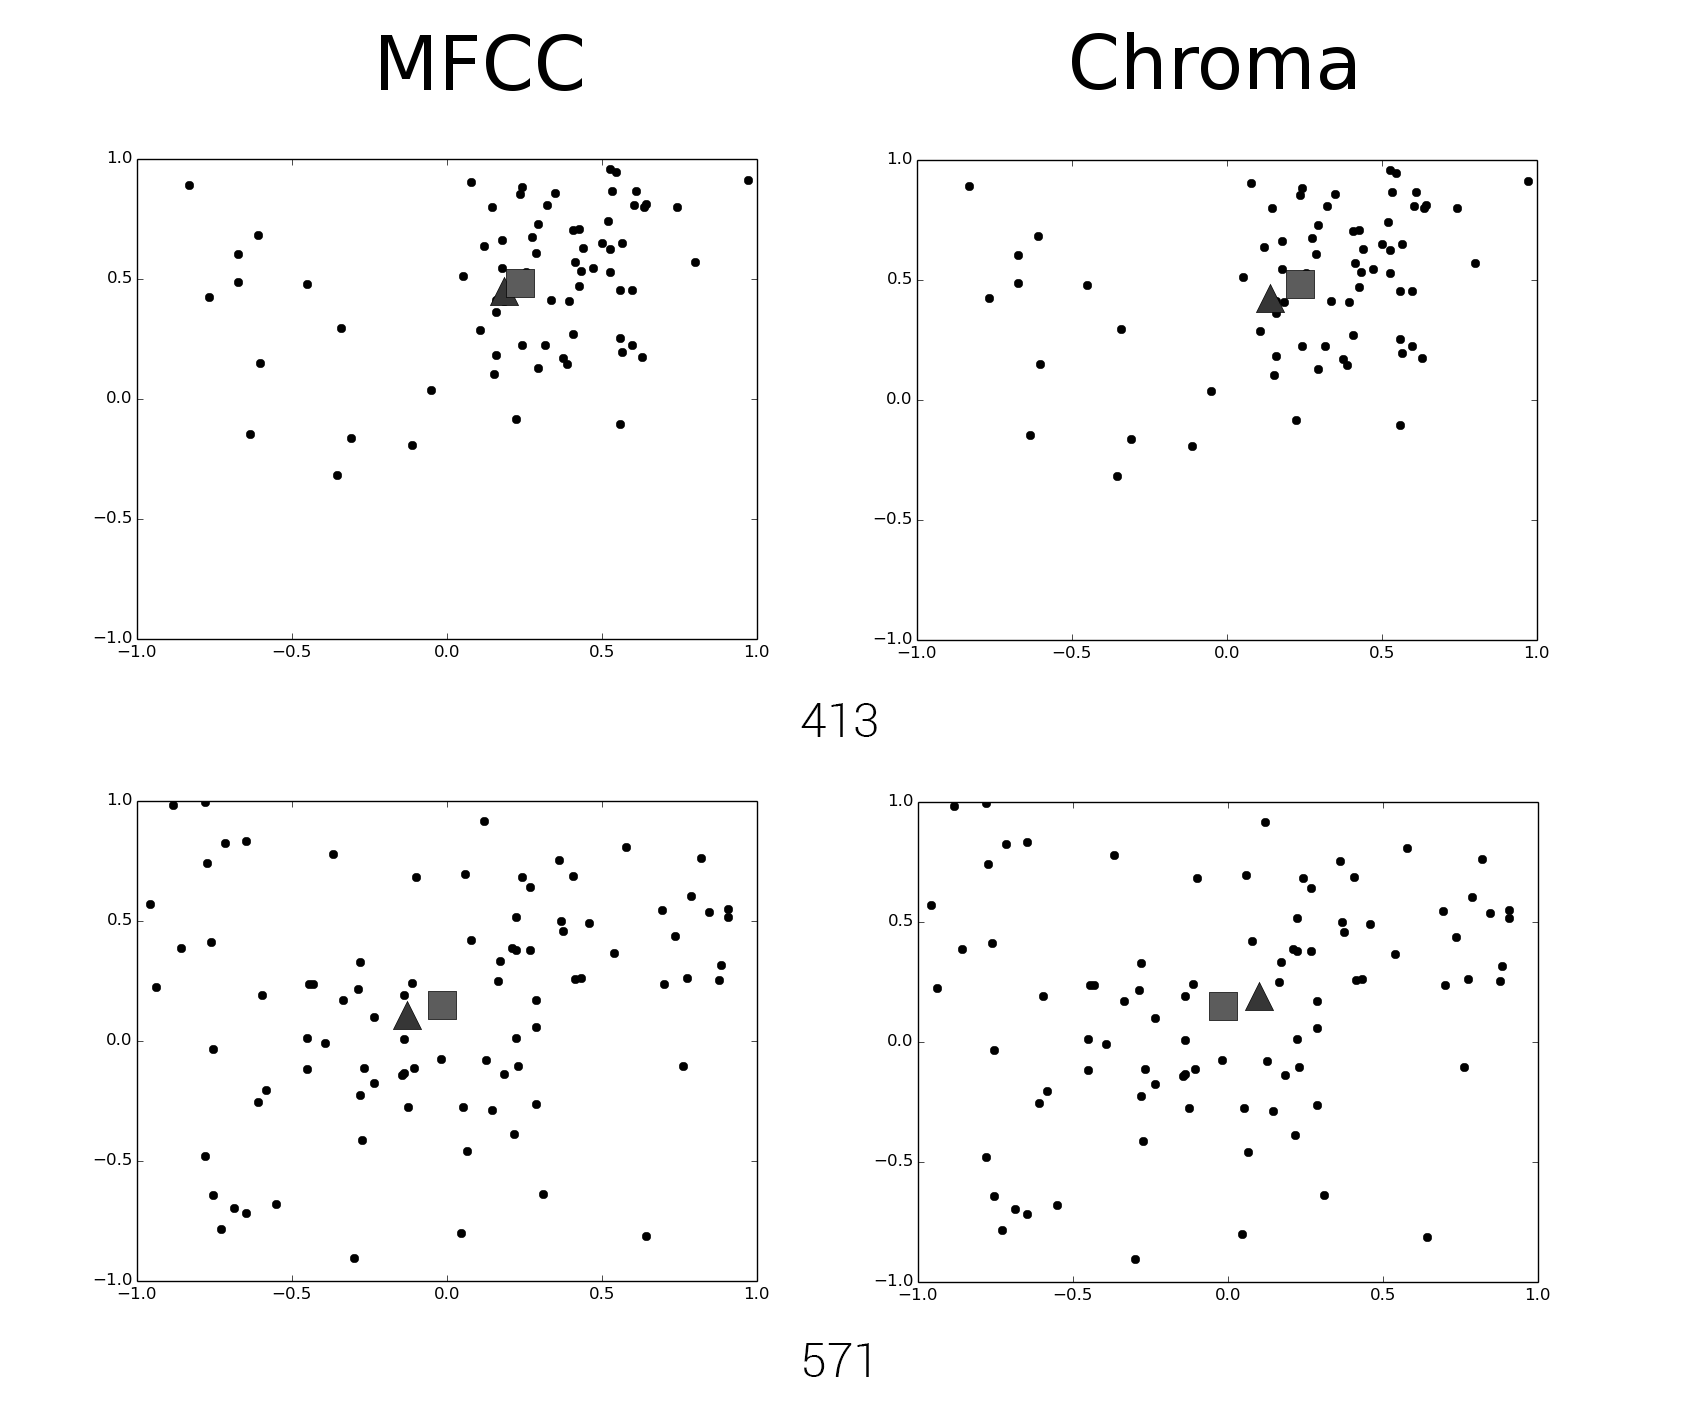
\includegraphics[width=130mm]{images/graphs1.png}
\caption{Slika predstavlja 4 VA prostore za pesmi z identifikacijskima številkama 413 (prva vrsta) in 571 (druga vrsta). Kvadrat predstavlja predstavlja povprečno vrednost iz podatkovne zbirke, trikotnik prikazuje napoved algoritma (z uporabo MFCC v prvem stolpcu in kromatskega vektorja v drugem). Pike prikazujejo posamezne vrednosti iz podatkovne zbirke.}
\label{graphs}
\end{figure}

V tabeli \ref{seperateresults} so predstavljene povprečne razdalje  izračunane ločeno za prijetnost (valence) in aktivnost (arousal). Iz teh rezultatov je razvidno, da je z uporabo vseh značilnic možno bolj natančno  napovedati aktivnost v primerjavi s prijetnostjo. Med tem je možno še opaziti, da kromatski vektor izračunan z Hierarhični kompozicionalnim modelom da veliko boljše rezultate pri računanju prijetnosti kot ostale značilnice, med tem ko je aktivnost izračunana podobno natančno kot z uporabo MFCC. 

Na podlagi značilnic je mogoče zelo dobro oceniti razpoloženje v VA prostoru. Najboljše napovedi, da značilnica kromatski vektor izračunan s hierarhičnim kompozicionalnim modelom. Ugotovili smo, da regresijski algoritem natančneje napoveduje aktivnost, kot prijetnost, kar kaže na to, da je aktivnost ali bolj direktno izražena v glasbi, ali jo je mogoče bolje zaznati iz izbranih značilnic. Glede na rezultate bi lahko zaključil, da algoritem, kljub ne najbolj točni napovedi dobro oceni predel prostora v katerem se nahaja razpoloženje. Natančnost bi lahko izboljšali z uporabo kombinacije več značilnic. Z nekaj izboljšavami bi lahko ta algoritem uporabili za ocenjevanje razpoloženja v priporočilnih sistemih.

\section{Essentia Gaiatransform algoritem}

Drugi algoritem, na katerem smo preizkusili natančnost napovedovanja razpoloženja na glasbenih odlomkih iz naše podatkovne zbirke, je GaiaTransform algoritem, ki na podlagi nekaterih značilnic izračuna nekatere visoko-nivojske značilnice \cite{bogdanov2013form}, med katerimi je tudi razpoloženje. Algoritem se nahaja v knjižnicah Essentia in Gaia \cite{bogdanov2013essentia}.

Essentia je knjižnica namenjena analizi zvoka in predvsem uporabi na MIR področju. Napisana je v C++ jeziku, možno pa jo je uporabiti tudi v jeziku Python. Ponuja funkcionalnost kot so branje in pisanje zvoka, standardno procesiranje signalov, statistična opredelitev podatkov, izračun velikega števila spektralnih, časovnih, tonskih in ostali značilnic. Te značilnice so osnova za izračun visoko nivojskih značilnic. Essentia skupaj s knjižnico Gaia ponuja funkcionalnosti za izračun nekaterih visoko nivojskih značilnic kot so žanr, kultura (zahodna ali nezahodna), vrsto plesa na izbrano skladbo, barvo zvoka, razpoloženja v skladbi. Ocenjuje tudi, ali je pesem inštrumental ali ne. Ker v tem delu preučujemo predvsem razpoloženje v glasbi, se bomo osredotočili na funkcionalnost, ki poskuša odkriti razpoloženje v glasbi.

Algoritem visoko nivojske značilnice izračuna na podlagi nizko nivojskih, ki so prav tako izračunane s knjižnico Essentia. Za določanje visoko nivojskih značilnic seveda ne uporabi vseh značilnic, ampak samo podmnožico teh. To podmnožico so za vsak razred (na primer srečo) izračunali posebej z uporabo algoritma za izbiro značilnic na podlagi korelacije (correlationbased feature selection - CFS). 

Za klasifikacijo so uporabili večrazredni (muliti-class) SVM algoritem z ena proti ena (one-versus-one) strategijo glasovanja (voting strategy). Uporabili so SVM algoritem iz knjižnice libSVM. Algoritem so razširili z možnostjo napovedovanja verjetnosti prisotnosti določenega razreda (na primer, da pove, da je verjetnost, da v pesmi nastopa sreča 89\%). SVM je naučen s petkratnim prečnim preverjanjem.  

Algoritem so naučili na 20 različnih glasbenih zbirkah. Algoritem za ocenjevanje razpoloženja iz glasbe so naučili na zbirki, ki so jo pripravili Laurier et. al \cite{Laurier2009}. Zbirko so potem sami še dodatno označili. 

Za razpoloženje algoritem vrne verjetnost, da je v neki pesmi prisotno eno od šestih razpoloženj: srečen (happy), žalosten (sad), agresiven (aggressive), sproščen (relaxed), akustičen (accoustic), elektronski (electronic) in zabaven (pary). Poleg tega pa algoritem glasbeni odlomek glede na razpoloženje razvrsti v enega od 5 gruč (clusters), ki so uporabljene v MIREX opravilu (MIREX task). Gruče so definirane s razpoloženji, ki spadajo v posamezno gruč. Razpoloženja, ki pripadajo posamezni gruči so predstavljena v tabeli \ref{mirextask2}.

\begin{table}[htb]
	\caption{Gruče razpoloženj, ki se uporabljajo v MIREX mood opravilu.}
    \begin{tabular}{|l|l|}
    \hline
    Gruče   & Razpoloženja  \\
    \hline                                                      
    Gruča 1 & strastno, vznemirjeno, razposajeno \\
    Gruča 2 & veselo, zabavno, prijetno, ljubeznivo \\
    Gruča 3 & ganljivo, bridko, potrto, otožno, grenko-sladko, malodušno  \\
    Gruča 4 & šaljivo, duhovito, smešno, neumno, čudaško, muhasto \\
    Gruča 5 & 
    \begin{tabular}[l]{@{}l@{}}
		agresivno, nasilno, ognjevito, razdražljivo, napeto,	intenzivno, \\
		 nestanovitno, spreminjajoče
	\end{tabular} \\
    \hline
    \end{tabular} 
    \label{mirextask2}   
\end{table}

\subsection{Natančnost razvrščanja}
\label{natancnostessentia}

Zgoraj opisani algoritem po podatkih avtorjev med samostojnimi oznakami za razpoloženje (vesel, žalosten, elektronski, zabaven, sproščen in agresiven) najbolje napoveduje prisotnost agresivnosti z natančnostjo 97,5\%. Temu sledijo razpoloženja sproščen (92,92\% natančno). Sledijo jima zabaven (88,38\%), žalosten (86,96\%) in elektronski (84,59\%). Najslabše napovedi da algoritem za razpoloženje vesel, kjer je natančnost 82,86\%.

\begin{table}[htb]
\begin{center}
\caption{Natančnost napovedovanja v gruče v odstotkih glede na teste, ki so jih naredili avtorji algoritma. V vrstici so gruče katerim pesem pripada, v stolpcu pa gruče kamor je algoritem uvrsti pesem.}
\begin{tabular}{|l|c|c|c|c|c|}
\hline
 & Gruča 1 & Gruča 2 & Gruča 3 & Gruča 4 & Gruča 5 \\ \hline
Gruča 1 & 58,62 & 18,97	& 10,34 & 3,45 & 8,62 \\ \hline
Gruča 2 & 29,63 & 48,15 & 16,67 & 5,56 & 0,00 \\ \hline
Gruča 3 & 10,81 & 13,51 & 71,62 & 4,05 & 0,00 \\ \hline
Gruča 4 & 15,62	& 43,75	& 12,50	& 25,00	& 3,12 \\ \hline
Gruča 5 & 25,49	& 1,96	& 0,00 & 1,96 & 70,59 \\ \hline

\hline
\end{tabular}
\label{natancnost_gruce}
\end{center}
\end{table}

Povsem drugačno je stanje pri natančnosti napovedovanja razpoloženj v gruče. V tem primeru je natančnost le  59.14\%. Iz tabele \ref{natancnost_gruce} je razvidno, da algoritem najbolj natančno napoveduje gručo 3 in gručo 5, najmanj natančno pa gručo 4. Iz tabele je tudi očitno, da sta gruča 2 in gruča 3 od gruče 5 tako drugačni, da ni napovedi, ki bi pesem namesto v gručo 2 ali gručo 3 uvrstila v gručo 5. Med tem pa je veliko napačnih preslikav med gručama 1 in 2. Veliko je tudi takšnih napačnih napovedi, ko algoritem pesmi namesto gruče 5 določi gručo 1. Obratna korelacija ni tako močna. 

\subsection{Rezultati napovedovanja z algoritmom Gaiatransform}

Primerjava rezultatov pri tem algoritmu je bila malo zahtevnejša kot primerjava z uporabo regresije, saj v naši podatkovni zbirki nimamo enakih oznak, kot jih algoritem vrača kot rezultat. Zaradi tega je bilo potrebno poenotiti oznake. Ugotovili smo, da bo primerjava najlažja, če uporabimo MIREX gruče, ki jih vrača algoritem. Oznake, ki jih imamo v naši podatkovni zbirki, smo razvrstili v gruče glede na podobnost z razpoloženji, ki se nahajajo v teh gručah in so prikazane v poglavju \ref{natancnostessentia}. Razporeditev razpoloženj iz naše podatkovne zbirke v gruče je prikazana v tabeli \ref{gruce_nase}. Opaziti je, da v četrto gručo nismo uvrstili nobenega razpoloženja iz naše podatkovne zbirke, ker se nobeno od razpoloženj ne ujema s tistimi na katerih je ta gruča definirana.

\begin{table}[htb]
\begin{center}
\caption{Razvrstitev oznak razpoloženja iz naše zbirke v MIREX gruče glede na podobnost z obstoječimi razpoloženji iz gruč. V četrti gruči ni nobenega razpoloženja, saj se nobeno razpoloženje iz naše zbirke ne ujema z razpoloženji iz te gruče.}
\begin{tabular}{|l|c|}
\hline
Gruča & Razpoloženja \\ \hline
Gruča 1 & presenečenje, navdihnjenost\\\hline
Gruča 2 & veselje, sreča, živahnost \\\hline
Gruča 3 & 
	\begin{tabular}[c]{@{}c@{}}
		žalost, otožnost, hrepenenje, pričakovanje.\\
		sproščenost, mirnost, zasanjanost
	\end{tabular}\\\hline
Gruča 4 & \\\hline
Gruča 5 & jeza, strah\\\hline

\hline
\end{tabular}
\label{gruce_nase}
\end{center}
\end{table}

Nato smo izvedli primerjavo tako, da smo pogledali katero je najbolj pogosto razpoloženje v podatkovni zbirki pri vsakem izmed 200 glasbenih odlomkov. To razpoloženje smo potem glede na preslikavo v tabeli \ref{gruce_nase} preslikal v gručo. V nadaljevanju smo te gruče primerjali z gručami, ki jih za isti glasbeni odlomek napove algoritem. 

\begin{table}[htb]
\begin{center}
\caption{Rezultati napovedovanja v gruče v odstotkih. V vrstici so gruče katerim pesem pripada, v stolpcu pa gruče kamor je algoritem uvrsti pesem. V četrti gruči so ničle, ker se nobeno razpoloženje iz naše zbirke ne ujema z razpoloženji iz te gruče. Zaradi tega tudi nobena pesem ne pripada tej gruči. Najbolj natančne ocene smo dobili za gručo 3, najslabše za gručo 1.}
\begin{tabular}{|l|c|c|c|c|c|c|}
\hline
 & Gruča 1 & Gruča 2 & Gruča 3 & Gruča 4 & Gruča 5 & Št. odl.\\ \hline
Gruča 1 & 14,29 & 14,29	& 57,14 & 0 & 14,29 & 7\\ \hline
Gruča 2 & 12,63 & 41,05 & 15,79 & 9,47 & 21,05 & 95\\ \hline
Gruča 3 & 8,86 & 25,32 & 58,22 & 1,27 & 6,33 & 79\\ \hline
Gruča 4 & 0	& 0 & 0 & 0 & 0 & 0\\ \hline
Gruča 5 & 26,32	& 5,26	& 15,79 & 5,26 & 47,37 & 19 \\ \hline

\hline
\end{tabular}
\label{natancnost_gruce_nasa}
\end{center}
\end{table}

Natančnost napovedovanja na naši podatkovni zbirki je 47,50\%. Bolj natančni rezultati napovedovanja so prikazani v tabeli \ref{natancnost_gruce_nasa}. Vsaka vrstica predstavlja gručo, v katero spada pesem. Stolpci pa predstavljajo gruče, v katere je algoritem uvrstil glasbeni odlomek. Torej na presečišču nam številka vrstice pove, kam bi moral spadati določen odlomek, številka stolpca pa kam ga je uvrstil algoritem. Na presečišču je zapisan odstotek elementov uvrščenih v gručo v stolpcu glede na število elementov v dejanski gruči. 

Iz teh podatkov je razvidno, da je algoritem najbolj natančno razvrstil elemente v gručo 3, medtem ko je bil najmanj natančen pri določanju gruče 1. Tukaj so rezultati slabi, saj je algoritem večino pesmi iz te gruče uvrstil v gručo 3. Mogoče je tukaj eden od problemov v tem, da je v tej gruči malo pesmi (7), zato ne moramo posplošiti teh rezultatov. V četrti vrstici so vsi rezultati nič, ker v naši podatkovni zbirki nimamo razpoloženja, za katerega bi lahko rekli, da pripada tej gruči. Tako ni nobene pesmi uvrščene v to gručo. Iz rezultatov lahko opazimo, da je več pesmi, ki so v gruči 5, algoritem uvrstil v gručo 1, kar je podobno rezultatom avtorjev algoritma prikazanim v poglavju \ref{natancnostessentia}. Z avtorjevimi rezultati je podobno tudi to, da odlomki iz gruče 1 niso bili uvrščeni v gručo 4 in to, da je bilo malo odlomkov iz gruče 5 uvrščeno v gručo 2.

Ker se pri določenih pesmih več razpoloženj pojavi skoraj enako pogosto v naši podatkovni zbirki, smo potem primerjavo dopolnili tako, da primerja vsa razpoloženja, ki so blizu razpoloženja, ki se pojavi največkrat. Če je gruča enega od teh razpoloženj enaka gruči, v katero je algoritem uvrstil glasbeni odlomek smatramo napoved kot pravilno. 

\begin{table}[htb]
\begin{center}
\caption{Rezultati napovedovanja v gruče v odstotkih v primeru, ko smo upoštevali tudi razpoloženja, ki so blizu največkrat označenem. V vrsticah so gruče, katerim pesem dejansko pripada, v stolpcu pa gruče kamor je algoritem uvrsti pesem. V četrto gručo nismo uvrstili nobene pesmi, zaradi neujemanja vseh naših razpoloženj z razpoloženji v tej gruči. Kot pri tabeli \ref{natancnost_gruce_nasa} so tudi tukaj najboljše napovedi za gručo 3 in najslabše za gručo 1. }
\begin{tabular}{|l|c|c|c|c|c|c|}
\hline
 & Gruča 1 & Gruča 2 & Gruča 3 & Gruča 4 & Gruča 5 & Št. odl.\\ \hline
Gruča 1 & 25 & 0	& 75 & 0 & 0 & 4\\ \hline
Gruča 2 & 12,37 & 44,33 & 15,46 & 9,28 & 18,56 & 97\\ \hline
Gruča 3 & 9,09 & 22,08 & 61,04 & 1,30 & 6,49 & 77\\ \hline
Gruča 4 & 0	& 0 & 0 & 0 & 0 & 0\\ \hline
Gruča 5 & 22,73	& 4,55 & 13,64 & 4,55 & 54,55 & 22 \\ \hline

\hline
\end{tabular}
\label{natancnost_gruce_nasa_with_second}
\end{center}
\end{table}

Pričakovano je bilo, da tak način natančnost napovedovanja poveča. Natančnost pridobljena na tak način znaša 51.5\%. Iz rezultatov v tabeli \ref{natancnost_gruce_nasa_with_second} je razvidno, da se je natančnost izražena v odstotkih najbolj povečala v prvi gruči, po številu pesmi pa v gruči 5. V gruči 1 so za razliko od prej samo še tiste napačne napovedi, ki se uvrščajo v gručo 3. Odstotek teh se je povečal, ker se je zmanjšalo skupno število pesmi v tej gruči. Ostale napovedi se niso bistveno spremenile. 

Kot smo že omenili algoritem poleg klasifikacije v MIREX gruče omogoča ocenjevanje za 6 razpoloženj. Za vsako od razpoloženj napove, če se pojavi v glasbenem odlomku. Glede na to, da se 3 od teh oznak ujemajo z oznakami v naši podatkovni zbirki, sem iz podatkovne zbirke vzel tiste pesmi, kjer je je to razpoloženje najbolj prisotno od vseh. Te pesmi sem potem primerjal z rezultati, ki jih vrne algoritem. 

\begin{table}[htb]
\begin{center}
\caption{Natančnost ocenjevanja razpoloženj vesel, žalosten in sproščen v odstotkih. Iz podatkov je razvidno, da algoritem na naši podatkovni zbirki zelo natančno oceni prisotnost razpoloženj žalosten in sproščen, slabši je pri ocenjevanju razpoloženja srečen. }
\begin{tabular}{|l|c|}
\hline
Srečen & 54,55\\ \hline
Žalosten & 86,36\\ \hline
Sproščen & 87,5\\ \hline

\end{tabular}
\label{natancnost_es_custva}
\end{center}
\end{table}

Za ta primer algoritem pravilno napove prisotnost razpoloženja s 79,59\% natančnostjo. Kot je razvidno iz tabele \ref{natancnost_es_custva} je natančnost velika pri razpoloženjih žalosten in sproščen. Dosti manjša pa je pri razpoloženju srečen, kar kaže na to, da je algoritmično direktno iz glasbenih odlomkov mnogo lažje napovedati sproščenost in žalost, medtem ko je to težje pri razpoloženju srečen. 

Z uporabo algoritma za določanje MIREX gruč iz Essentie smo na naši podatkovni zbirki dobili slabše rezultate, kot so jih dobili avtorji. To gre po vsej verjetnosti pripisati temu, da naše oznake niso enake tistim, ki jih vrača algoritem, pri ročni pretvorbi pa nismo mogli zagotoviti popolnega ujemanja. 

Pri napovedovanju posameznega razpoloženja so rezultati približno enaki tistim, ki so jih dobili avtorji za razpoloženji žalosten in sproščen. Za razpoloženje vesel so rezultati slabši. Mogoče gre za razliko v dojemanju razpoloženja srečen v slovenščini in razpoloženja "happy" v angleščini. 

%%%%%%%%%%%%%%%%%%%%%%%%%%%%%%
%% poglaje					%%
%%%%%%%%%%%%%%%%%%%%%%%%%%%%%%
\chapter{Napovedovanje razpoloženja iz barve}

Pri zbiranju podatkovne zbirke smo, poleg razpoloženja, zajemali podatke o tem, s kakšno barvo bi udeleženec opisal razpoloženje v glasbenem odlomku. V poglavju \ref{razcusbar} smo ugotovili, da obstaja povezava med barvami in razpoloženjem. To povezavo smo uporabili za ocenjevanje razpoloženja na podlagi podatkov o barvi. Napovedovali smo prijetnost in aktivnost. Obenem smo preizkusili tudi obratno povezavo, tako da smo ocenjevali barvo posameznega glasbenega odlomka na podlagi podatkov o razpoloženju. Za ocenjevanje razpoloženja iz barve in obratno, smo se odločili, da pokažemo obstoj korelacije med barvami in razpoloženjem v glasbenem odlomku. Ta povezava je koristna za povečanje natančnosti ocenjevanja razpoloženja z algoritmom, ki ga bomo implementirali v prihodnosti in pri vizualizaciji glasbe z barvami.

Za ocenjevanje razpoloženja in barve, smo uporabili regresijski algoritem podoben tistemu, opisanem v poglavju \ref{regresijsialg} z nekaj spremembami. Namesto značilnic smo uporabili podatke o barvi ali podatke o razpoloženju. Algoritem smo izvajali na vseh tipičnih odzivih za izražena čustva v podatkovni zbirki. Tipični odzivi so tisti, ki imajo za glasbeni odlomek samo eno VA oznako. Za izbiro tipičnih odzivov smo se odločili, ker edino pri teh vemo, katero je najbolj značilno razpoloženje za glasbeni odlomek glede na mnenje posameznega udeleženca. Pri odzivih z več izraženimi razpoloženji ni možno določiti, katero je najbolj značilno. Tipičnih odzivov v naši podatkovni zbirki je 2950, kar je 41\% vseh odzivov. 

Za preizkus smo pri vsakem odzivu uporabili podatek o barvi zapisani v HSV barvnem prostoru in podatek o razpoloženju zapisanem v VA prostoru. HSV zapis \cite{Sural2002} vsebuje tri komponente odtenek (hue - H), intenzivnost (staturation - S) in svetlost (value - V). Barvo iz HSV barvnega modela smo pretvorili tudi v RGB zapis \cite{susstrunk1999standard} in poskusili ocenjevanje razpoloženja iz tega zapisa. Prav tako smo iz kartezičnih koordinat za razpoloženje izračunali polarne \cite{julier1997consistent} in preizkusili ocenjevanje na teh. Za izbiro polarnega koordinatnega sistema smo se odločili, ker smo želeli preveriti, če obstaja tudi korelacija med barvo in razpoloženjem zapisanem s polarnimi koordinatami. 

\section{Rezultati napovedovanja razpoloženja iz barve}

Iz rezultatov v tabeli \ref{colormoodreg} je razvidno, da je možno zelo napovedati razpoloženje, zapisano v kartezičnih in polarnih koordinatah, iz barve zapisane v HSV barvnem modelu. Malo slabše so napovedi kartezičnih vrednosti za razpoloženje iz RGB barvnega zapisa, med tem ko napovedovanje razpoloženja v polarnem zapisu iz RGB modela ne prinese dobrih napovedi. Opazno je, da je pri napovedovanju razpoloženja v kartezičnem zapisu, veliko lažje oceniti aktivnost kot prijetnost, kar se je izkazalo že pri algoritmu v poglavju \ref{regresijsialg}. 

Ocene razpoloženja v polarnih koordinatah so natančnejše, kot tiste v kartezičnem koordinatnem sistemu, čeprav na prvi pogled ne zgleda tako. Potrebno je upoštevati, da je obseg ocen v tem primeru drugačen. Če gledamo odmik od povprečne vrednosti v razmerju z obsegom vrednosti opazimo, da je v tem primeru razmerje manjše, kar pomeni bolj točne napovedi. Pri polarnem zapisu je napoved za $r$ vrednost bolj natančna kot napoved za $\varphi$. To kaže na to, da je možno bolj natančno napovedati odmik od središča koordinatnega sistema, kot kot med vektorjema, ki kažete iz izhodišča proti točkam z ocenami.

Pri ocenjevanju barve iz razpoloženja je razvidno, da so napovedi za HSV barvni model iz kartezičnih koordinat slabe, medtem ko so rezultati z uporabo polarnih koordinat boljši. To se je izkazalo že pri napovedih razpoloženja iz barve. Na podlagi tega lahko sklepamo na boljšo korelacijo med tema komponentama. Napovedi za hue (odtenek) so v obeh primerih boljše kot napovedi za value (svetlost), med tem ko so rezultati za saturation (intenzivnost) tako naključni, da so v tabeli izpuščeni. Pri napovedovanju barve v RGB barvnem modelu so edine smiselne napovedi za komponento blue (modro), čeprav tudi te v nobenem primeru ne kažejo velike korelacije med razpoloženjem in RGB zapisom barve. 

\begin{table}[hbt]
\begin{center}

\caption{Rezultati natančnosti ocenjevanja razpoloženja iz barve in barve iz razpoloženja z regresijskim algoritmom. Prikazni so le rezultati, ki kažejo določeno povezavo. Tam kjer ni povezave so vrednosti zelo naključne. Prikazana je povprečna razdalja do povprečnih vrednosti za posamezno pesem v zbirki. VA$_{x,y}$ je oznaka za razpoloženje v VA prostoru zapisano s kartezičnimi koordinatami, VA$_{r,\varphi}$ je zapis za razpoloženje v VA prostoru zapisano s polarnimi koordinatami. Podatkom je dodan obseg vrednosti ocenjenega parametra, da si lahko predstavljamo, kako natančne so ocene. }

\begin{tabular}{|l|l|l|}
\hline
\textbf{Način napovedovanja} & \textbf{Povprečna razdalja} & \textbf{Obseg vrednosti} \\ \hline
Ocenjevanje HSV iz VA$_{x,y}$ & 
	\begin{tabular}[l]{@{}l@{}}
		hue: 0.2697 \\
		value: 0.6486
	\end{tabular} &
	\begin{tabular}[l]{@{}l@{}}
		hue: [0, 1] \\
		value: [0,1]
	\end{tabular}
\\ \hline
Ocenjevanje RGB iz VA$_{x,y}$ & 
	\begin{tabular}[l]{@{}l@{}}
		blue: 0.4346
	\end{tabular} &
	blue: [0, 1]
\\ \hline
Ocenjevanje VA$_{x,y}$ iz HSV & 
	\begin{tabular}[l]{@{}l@{}}
		valence: 0.2000 \\
		arousal: 0.1279
	\end{tabular} &
	\begin{tabular}[l]{@{}l@{}}
		valence: [-1, 1] \\
		arousal: [-1,1]
	\end{tabular}
\\ \hline
Ocenjevanje VA$_{x,y}$ iz RGB & 
	\begin{tabular}[l]{@{}l@{}}
		valence: 0.2206 \\
		arousal: 0.1887
	\end{tabular} &
	\begin{tabular}[l]{@{}l@{}}
		valence: [-1, 1] \\
		arousal: [-1,1]
	\end{tabular}
\\ \hline


Ocenjevanje HSV iz VA$_{r,\varphi}$ & 
	\begin{tabular}[l]{@{}l@{}}
		hue: 0.1431 \\
		value: 0.3215
	\end{tabular} &
	\begin{tabular}[l]{@{}l@{}}
		hue: [0, 1] \\
		value: [0,1]
	\end{tabular}
\\ \hline
Ocenjevanje RGB iz VA$_{r,\varphi}$ & 
	\begin{tabular}[l]{@{}l@{}}
		blue: 0.2265
	\end{tabular} &
	blue: [0, 1]
\\ \hline
Ocenjevanje VA$_{r,\varphi}$ iz HSV & 
	\begin{tabular}[l]{@{}l@{}}
		r: 0.1083 \\
		$\varphi$: 0.3092
	\end{tabular} &
	\begin{tabular}[l]{@{}l@{}}
		r: [0, $\sqrt{2}$] \\
		$\varphi$: [0, $2\pi$]
	\end{tabular}
\\ \hline
Ocenjevanje VA$_{r,\varphi}$ iz RGB & 
	\begin{tabular}[l]{@{}l@{}}
		r: 0.2934 \\
		$\varphi$: 0.4166
	\end{tabular} &
	\begin{tabular}[l]{@{}l@{}}
		r: [0, $\sqrt{2}$] \\
		$\varphi$: [0, $2\pi$]
	\end{tabular}
\\ \hline

\end{tabular}
\end{center}
\label{colormoodreg}
\end{table}

Če podatke primerjamo z ocenami na podlagi značilnic MFCC in kromatski vektor ugotovimo, da so nekatere ocene skoraj tako dobre, kot tiste predstavljene v poglavju  \ref{regressionresults}. Razdalja od povprečja pri ocenah razpoloženja, izračunanih na podlagi barve zapisane v HSV barvnem modelu, se pri valence komponenti s tisto izračunano na podlagi kromatskega vektorja razlikuje za manj kot 0,02, pri aktivnosti je večja le za 0,03. V primerjavi z ocenami za MFCC in HKM kromatski vektor, je razlika malo večja. Prav tako opazimo podobnost v natančnosti ocen za prijetnost in aktivnost. V obeh primerih algoritem veliko lažje oceni aktivnost, kot prijetnost.

Ugotovili smo, da je mogoče na podlagi podatka o barvi z razmeroma dobro natančnostjo oceniti razpoloženje v primerjavi z ocenami na podlagi značilnic. To nam odpira možnosti za izboljšanje algoritmov za ocenjevanje čustev iz glasbe z dodatnimi parametri, ki niso pridobljeni direktno iz glasbe. Prav tako je pomembna obratna povezava. Na podlagi razpoloženja je mogoče dobro oceniti odtenek v barvnem prostoru HSV. Čeprav je ta napoved slabša od tiste za razpoloženje, nam pove pravi odtenek ali zelo sorodnega, saj so v HSV barvnem prostoru podobni odtenki glede na vrednost parametra hue skupaj. Ta podatek nam koristi pri vizualizaciji glasbe z barvami.

\chapter{Zaključek in nadaljnje delo}

Zbrali smo podatkovno zbirko s pomočjo spletne ankete. Zbirka vključuje veliko število odgovorov in bo kmalu na javno objavljena. Podatkovna zbirka vključuje udeleženčeve demografske podatke, podatke o njegovi percepciji razpoloženja in barv ter najbolj pomembno veliko razpoloženjskih in barvnih oznak za glasbene odlomke. Ti vključujejo razpoloženja, ki jih glasba vzbudi pri uporabniku in razpoloženja, ki se po udeleženčevem mnenju pojavijo v glasbenem odlomku skupaj z VA vrednostmi. Vsak odgovor vsebuje tudi podatek o barvi, ki po uporabnikovem mnenju najbolje opisujejo razpoloženje v glasbenem odlomku. Za razliko od nekaterih ostalih podatkovnih zbirk naša vključuje tudi glasbene odlomke. Ta podatkovna zbirka odpira nove možnosti za raziskovanje ocenjevanja čustev iz glasbe.  

Uporabili smo dva algoritma za ocenjevanje čustev iz glasbe. Prvi je regresijski algoritem, ki napoveduje prijetnost in aktivnost na podlagi značilnic MFCC in kromatski vektor. Najboljše rezultate dobimo če uporabimo kromatski vektor izračunan s hierarhičnim kompozicionalnim modelom \cite{Pesek2013}. Ugotovili smo tudi, da je aktivnost možno napovedati z večjo natančnostjo kot prijetnost. Drugi algoritem je Gaiatransforma algoritem, ki glasbene odlomke, glede na razpoloženje, klasificira v 5 gruč določenih s strani MIREX-a. Algoritem na naši podatkovni zbirki ocenjuje razpoloženje s približno polovično natančnostjo. Z največjo natančnostjo klasificira v gručo 3, ki vsebuje razpoloženja: žalost, otožnost, hrepenenje, pričakovanje, sproščenost, mirnost in zasanjanost. Najslabše klasificira v gručo 1 z razpoloženji presenečenje in navdihnjenost. Poleg kasifikacije v gruče algoritem ocenjuje pristnost razpoloženj sreča, žalost in sproščenost, kjer prisotnost razpoloženja sproščenost na naši zbirki ocenjuje z 87,5\% natančnostjo. Zelo dobro ocenjuje tudi pristnost razpoloženja žalost, pri sreči so rezultati slabši. 

Za konec smo preizkusili še uporabnost ostalih podatkov iz zbirke. Preizkusili smo natančnost ocenjevanja razpoloženja na podlagi barve za glasbene odlomke iz zbirke in obratno. Izkazalo se je, da je možno na podlagi HSV zapisa za barvo možno zelo dobro napovedati razpoloženje, pri čemer z večjo natančnostjo ocenimo arousal komponento. Možno je tudi dobro oceniti hue komponento za barvo na podlagi polarnega zapisa koordinat za VA vrednost. 

Ocenjevanje čustev iz glasbe je pomembna osnova za različna opravila vključujoč priporočilne sisteme za glasbo na podlagi razpoloženja. Uporabnikovi podatki v naši podatkovni zbirki prinesejo nove možnosti za raziskovanje uporabnosti teh podatkov v priporočilnih sistemih.

Kmalu bomo začeli z izvajanjem drugega kroga ankete, ki bo izvedena tudi v angleškem jeziku. Vsebovala bo dodatno zbirko glasbenih odlomkov. S tem želimo povečati število odgovorov na glasbeni odlomek in povečati število odlomkov v podatkovni zbirki. Pridobljeni podatki nam bodo dali možnost primerjave podatkov med udeleženci, ki govorijo slovensko in ostalimi. Nadaljevali bomo s testiranjem algoritmov za ocenjevanje čustev iz glasbe. Načrtujemo razviti novo metodo za ocenjevanje čustev iz glasbe, ki bo upoštevala tudi demografske in ostale podatke iz zbirke. 

V nadaljevanju bomo še bolj raziskali povezavo med razpoloženjem in barvami. Načrtujemo narediti vizualizacijo za podlagi rezultatov te raziskave. Vizualizacija bo uporabljena v vmesniku priporočilnega sistema na podlagi razpoloženja, ki ga nameravamo razviti.   


\bibliography{diploma1}{}
\bibliographystyle{unsrt}

\end{document}

